% $Header: /Users/joseph/Documents/LaTeX/beamer/solutions/conference-talks/conference-ornate-20min.en.tex,v 90e850259b8b 2007/01/28 20:48:30 tantau $

\documentclass[xcolor={usenames,dvipsnames}, aspectratio=169]{beamer}

% This file is a solution template for:

% - Talk at a conference/colloquium.
% - Talk length is about 20min.
% - Style is ornate.



% Copyright 2004 by Till Tantau <tantau@users.sourceforge.net>.
%
% In principle, this file can be redistributed and/or modified under
% the terms of the GNU Public License, version 2.
%
% However, this file is supposed to be a template to be modified
% for your own needs. For this reason, if you use this file as a
% template and not specifically distribute it as part of a another
% package/program, I grant the extra permission to freely copy and
% modify this file as you see fit and even to delete this copyright
% notice. 


\mode<presentation>
{
  \usetheme{AnnArbor}

  \setbeamercovered{transparent}
  % or whatever (possibly just delete it)
 }

\usepackage[percent]{overpic}
\usepackage[english]{babel}
\usepackage{multirow}
\usepackage[at]{easylist}
\usepackage{appendixnumberbeamer}
\usepackage{bm}
\usepackage{setspace}
% or whatever

\usepackage[latin1]{inputenc}
% or whatever

\usepackage{times}
\usepackage[T1]{fontenc}
% Or whatever. Note that the encoding and the font should match. If T1
% does not look nice, try deleting the line with the fontenc.
%particles
\newcommand{\jpsi}{\rm J/$\psi$}
\newcommand{\psip}{$\psi^\prime$}
\newcommand{\jpsiDY}{\rm J/$\psi$\,/\,DY}
\newcommand{\chic}{$\chi_{\rm c}$}
\newcommand{\pip}{$\pi^{+}$}
\newcommand{\pim}{$\pi^{-}$}
\newcommand{\pizero}{$\pi^{0}$}
\newcommand{\kap}{K$^{+}$}
\newcommand{\kam}{K$^{-}$}
\newcommand{\pbar}{$\rm\overline{p}$}
\newcommand{\ccbar}{\ensuremath{\mathrm{c\overline{c}}}}
\newcommand{\bbbar}{\ensuremath{\mathrm{b\overline{b}}}}
\newcommand{\Dzero}{\ensuremath{\mathrm{D^{0}}}}
\newcommand{\Dzerobar}{\ensuremath{\mathrm{\overline{D}^{0}}}}
\newcommand{\Dpm}{\ensuremath{\mathrm{D^{\pm}}}}
\newcommand{\Ds}{\ensuremath{\mathrm{D_{s}^{\pm}}}}
\newcommand{\Dstar}{\ensuremath{\mathrm{D^{*\pm}}}}

%collision systems
\newcommand{\pp}{pp}
\newcommand{\pPb}{p--Pb}
\newcommand{\PbPb}{Pb--Pb}

%detectors
\newcommand{\ezdc}{$E_{\rm ZDC}$}

%units
\newcommand{\GeVc}{GeV/$c$}
\newcommand{\GeVcsq}{GeV/$c^2$}

%others
\newcommand{\degree}{$^{\rm o}$}
\newcommand{\s}{\ensuremath{\sqrt{s}}}
\newcommand{\snn}{\ensuremath{\sqrt{s_{\rm NN}}}}
\newcommand{\y}{\ensuremath{y}}
\newcommand{\pt}{\ensuremath{p_{\rm T}}}
\newcommand{\dedx}{d$E$/d$x$}
\newcommand{\dndy}{d$N$/d$y$}
\newcommand{\dndydpt}{${\rm d}^2N/({\rm d}y {\rm d}p_{\rm t})$}
\newcommand{\zpar}{\ensuremath{z_{||}}}
\newcommand{\zpargen}{\ensuremath{z_{||}^{\mathrm{part}}}}
\newcommand{\zpardet}{\ensuremath{z_{||}^{\mathrm{det}}}}
\newcommand{\ptchjet}{\ensuremath{p_{\mathrm{T,ch\, jet}}}}
\newcommand{\ptjet}{\ensuremath{p_{\mathrm{T,jet}}}}
\newcommand{\ptchjetgen}{\ensuremath{p_{\mathrm{T,ch\,jet}}^{\mathrm{part}}}}
\newcommand{\ptchjetdet}{\ensuremath{p_{\mathrm{T,ch\,jet}}^{\mathrm{det}}}}
\newcommand{\ptd}{\ensuremath{p_{\mathrm{T,D}}}}
\newcommand{\ptdgen}{\ensuremath{p_{\mathrm{T,D}}^{\mathrm{part}}}}
\newcommand{\ptddet}{\ensuremath{p_{\mathrm{T,D}}^{\mathrm{det}}}}
\newcommand{\antikt}{anti-\ensuremath{k_{\mathrm{T}}}}
\newcommand{\Antikt}{Anti-\ensuremath{k_{\mathrm{T}}}}
\newcommand{\kt}{\ensuremath{k_{\mathrm{T}}}}
\newcommand{\pthard}{\ensuremath{p_{\mathrm{T,hard}}}}

\AtBeginSection[]{
  \begin{frame}
  \vfill
  \centering
  \begin{beamercolorbox}[sep=8pt,center,shadow=true,rounded=true]{title}
    \usebeamerfont{title}\insertsectionhead\par%
  \end{beamercolorbox}
  \vfill
  \end{frame}
}

\title[D-Tagged Jets in \pp\ and \pPb] % (optional, use only with long paper titles)
{D-Tagged Jets in \pp\ and \pPb\ collisions}

\author[Salvatore Aiola]% (optional, use only with lots of authors)
{Salvatore Aiola (Yale University) \\
Barbara Trzeciak (Utrecht University) \\
Auro Mohanty (Utrecht University)
}
% - Give the names in the same order as the appear in the paper.
% - Use the \inst{?} command only if the authors have different
%   affiliation.

\institute[Yale University] % (optional, but mostly needed)
{}

\date[Jan. 26th, 2018] % (optional, should be abbreviation of conference name)
{PAG-HFCJ and PWG-JE joint meeting\\
January 26th, 2018}
% - Either use conference name or its abbreviation.
% - Not really informative to the audience, more for people (including
%   yourself) who are reading the slides online

\subject{High-Energy Physics}
% This is only inserted into the PDF information catalog. Can be left
% out. 



% If you have a file called "university-logo-filename.xxx", where xxx
% is a graphic format that can be processed by latex or pdflatex,
% resp., then you can add a logo as follows:

% \pgfdeclareimage[height=0.5cm]{university-logo}{university-logo-filename}
% \logo{\pgfuseimage{university-logo}}


% If you wish to uncover everything in a step-wise fashion, uncomment
% the following command: 

%\beamerdefaultoverlayspecification{<+->}

\begin{document}

\begin{frame}
  \titlepage
\end{frame}

%\begin{frame}{Outline}
  %  \tableofcontents
%\end{frame}


% Structuring a talk is a difficult task and the following structure
% may not be suitable. Here are some rules that apply for this
% solution: 

% - Exactly two or three sections (other than the summary).
% - At *most* three subsections per section.
% - Talk about 30s to 2min per frame. So there should be between about
%   15 and 30 frames, all told.

% - A conference audience is likely to know very little of what you
%   are going to talk about. So *simplify*!
% - In a 20min talk, getting the main ideas across is hard
%   enough. Leave out details, even if it means being less precise than
%   you think necessary.
% - If you omit details that are vital to the proof/implementation,
%   just say so once. Everybody will be happy with that.

%\begin{overpic}[width=.85\textwidth, trim=0 0 0 0, clip]{img/ReflectionTemplates_DPt_NoJet_DoubleGaus_1010}
%\put(0,61){{\tiny No jet requirement}}
%\put(60,61){{\tiny \textcolor{ForestGreen}{\textbf{Used for QM17 preliminary}}}}
%\end{overpic}

%\begin{columns}
%\column{0.5\textwidth}
%\column{0.5\textwidth}
%\end{columns}

\section{\pp\ collisions at $\s=7$~TeV}

\subsection{Physics Results and Discussion}

\begin{frame}[t]{Momentum Fraction Distribution}
\begin{columns}[t]
\column{0.30\textwidth}
\centering
\footnotesize
$5<\ptchjet<15$~\GeVc\\
$\ptd>2$~\GeVc\\
\begin{overpic}[width=1.07\textwidth, trim=0 0 0 0, clip]{img/paper_figures/JetZSpectrum_JetPt_5_15_Paper}
\end{overpic}\\
\only<3>{
\scriptsize
$\overline{z}_{\rm data}=0.765 \pm 0.014$\\
$\overline{z}_{\rm theory}=0.785 \pm 0.004$\\
p-value$=0.41$ (full distribution)
}
\column{0.30\textwidth}
\centering
\footnotesize
$15<\ptchjet<30$~\GeVc\\
$\ptd>6$~\GeVc\\
\begin{overpic}[width=1.07\textwidth, trim=0 0 0 0, clip]{img/paper_figures/JetZSpectrum_JetPt_15_30_Paper}
\end{overpic}\\
\only<3>{
\scriptsize
$\overline{z}_{\rm data}=0.710 \pm 0.028$\\
$\overline{z}_{\rm theory}=0.747 \pm 0.005$\\
p-value$=0.08$ (full distribution)
}
\column{0.38\textwidth}
\vspace{-20pt}
\begin{center}
$\zpar=\frac{\boldsymbol{p}_{\rm ch\,jet} \cdot \boldsymbol{p}_{\rm D}}{\boldsymbol{p}_{\rm ch\,jet} \cdot \boldsymbol{p}_{\rm ch\,jet}}$
\end{center}
\footnotesize
\begin{itemize}
\only<1>{
\item \antikt, $R=0.4$, $|\eta_{\rm jet}|<0.5$
\item Invariant mass analysis: side-band subtraction in \ptd\ bins
\item Corrections applied: reconstruction efficiency, B feed-down, unfolding of the detector momentum fraction resolution
\item Full systematics (see details in the following slides)
}
\only<2>{
\item The fragmentation looks quite different for the two \ptchjet\ ranges
\item Peak at $\zpar\approx1$ due to single-particle jets not present for intermediate jet momenta
}
\only<3>{
\item Theory: POWHEG+PYTHIA6
\item The systematic uncertainty on the MC distribution is small because the overall normalization does not matter
\item Data supports a slightly softer fragmentation compared to theory in the intermediate jet momentum (about 1-$\sigma$ discrepancy)
\item To do: separate different production mechanisms in MC
}
\end{itemize}
\end{columns}
\only<1>{
\vspace{10pt}
\footnotesize
Distributions are normalized to $1$ and each bin content divided by the corresponding bin width
}
\end{frame}

\subsection{Raw Yield Extraction}

\begin{frame}{Raw Yield Extraction: $5<\ptchjet<15$~\GeVc}
\begin{columns}
\column{0.33\textwidth}
\centering
\begin{overpic}[width=\textwidth, trim=0 0 0 0, clip]{img/raw_yield_z/AnyINT_D0_D0toKpiCuts_Charged_R040_DPtBins_JetPt_5_15_SideBand_D0_D0toKpiCuts_Charged_R040_JetZSpectrum_DPt_20_JetPt_5_15_SideBand}
\end{overpic}
\column{0.33\textwidth}
\centering
\begin{overpic}[width=\textwidth, trim=0 0 0 0, clip]{img/raw_yield_z/AnyINT_D0_D0toKpiCuts_Charged_R040_JetZSpectrum_DPt_20_JetPt_5_15_SideBand_BkgVsSig}
\end{overpic}
\column{0.33\textwidth}
\centering
\begin{overpic}[width=\textwidth, trim=0 0 0 0, clip]{img/raw_yield_z/AnyINT_D0_D0toKpiCuts_Charged_R040_JetZSpectrum_DPt_20_JetPt_5_15_SideBand_TotalBkgVsSig}
\end{overpic}
\end{columns}
\vspace{5pt}
\centering
$\textcolor{NavyBlue}{N_{\rm raw}(\zpar)}=\sum_{\ptd}\frac{1}{\epsilon\left(\ptd\right)}\left(\textcolor{BrickRed}{N_{\rm sig}(\zpar,\ptd)}-\frac{S}{B}\textcolor{ForestGreen}{N_{\rm SB}(\zpar,\ptd)}\right)$
\end{frame}

\subsection{B Feed-Down}

\begin{frame}{B Feed-Down Subtraction}
\begin{columns}
\column{0.33\textwidth}
\centering
\footnotesize
$5<\ptchjet<15$~\GeVc\\
\begin{overpic}[width=\textwidth, trim=0 0 0 0, clip]{img/b_feed_down/BFeedDown_JetZSpectrum_JetPt_5_15_InternalPlot}
\end{overpic}
\column{0.30\textwidth}
\centering
\footnotesize
$15<\ptchjet<30$~\GeVc\\
\begin{overpic}[width=1.1\textwidth, trim=0 0 0 0, clip]{img/b_feed_down/BFeedDown_JetZSpectrum_JetPt_15_30_InternalPlot}
\end{overpic}
\column{0.37\textwidth}
\small
\begin{itemize}
\item Folded with detector response (jet momentum resolution)
\item Multiplied by the ratio of the $\epsilon_{\rm non-prompt} / \epsilon_{\rm prompt}$
\item Multiply by the $L_{\rm int}$ and subtract from efficiency-corrected raw yields
\item Feed-down between $10-35$\%
\end{itemize}
\end{columns}
\centering
\footnotesize
\vspace{10pt}
$\textcolor{ForestGreen}{N_{\rm sub}(\zparreco)} = \textcolor{NavyBlue}{N_{\rm raw}(\zparreco)} - \textcolor{BrickRed}{L_{\rm int} \int_{\zpar,\ptd}\left[\frac{\epsilon_{\rm non-prompt}(\ptd)}{\epsilon_{\rm prompt}(\ptd)} R_{\rm det}^{\rm non-prompt}(\zpar,\zparreco) \cdot \frac{d^2\sigma_{\rm POWHEG}}{d\zpar d\ptd}\right]} $
\end{frame}

\subsection{Unfolding}

\begin{frame}[t]{Bayesian Unfolding: $5<\ptchjet<15$~\GeVc}
\begin{columns}
\column{0.36\textwidth}
\scriptsize
\centering
Response Matrix\\
\begin{overpic}[width=\textwidth, trim=0 240 290 0, clip]{img/unfolding/JetZ_SideBand_DPt_20_JetPt_5_15_Response_PriorResponseTruth}
\end{overpic}\\ 
\scriptsize
Good resolution (color log scale!)\\
$\sim10$~\% off diagonal
\column{0.30\textwidth}
\centering
\begin{overpic}[width=\textwidth, trim=0 0 0 0, clip]{img/unfolding/JetZ_SideBand_DPt_20_JetPt_5_15_UnfoldingSummary_Bayes}
\end{overpic}\\
\scriptsize
\centering
\textcolor{NavyBlue}{Unfolded / Measured}\\
\vspace{2pt}
\begin{overpic}[width=1.13\textwidth, trim=0 0 0 0, clip]{img/unfolding/JetZ_SideBand_DPt_20_JetPt_5_15_UnfoldingSummary_Bayes_UnfoldedOverMeasured}
\end{overpic}
\column{0.34\textwidth}
\scriptsize
\centering
\textcolor{ForestGreen}{Refolded / Measured}\\
\begin{overpic}[width=\textwidth, trim=0 0 0 0, clip]{img/unfolding/JetZ_SideBand_DPt_20_JetPt_5_15_UnfoldingSummary_Bayes_RefoldedOverMeasured}
\end{overpic}
Good agreement \textcolor{ForestGreen}{refolded / measured} \\
\vspace{5pt}
Statistical uncertainties (fluctuations) are ``regularized'' in unfolded solution ($7$\% deviation in the first bin)\\
\vspace{5pt}
Overall a small correction, up to $\sim6$\% (see \textcolor{NavyBlue}{Unfolded/Measured})
\end{columns}
\end{frame}

\begin{frame}[fragile]{Unfolding Stability: $5<\ptchjet<15$~\GeVc}
\begin{columns}
\column{0.32\textwidth}
\centering
\tiny 
Number of iterations (Bayes)\\
\begin{overpic}[width=\textwidth, trim=0 0 0 0, clip]{img/unfolding/JetZ_SideBand_DPt_20_JetPt_5_15_UnfoldingRegularization_Bayes_PriorResponseTruth_Ratio}
\end{overpic}\\
\tiny
Unfolding method\\
\begin{overpic}[width=\textwidth, trim=0 0 0 0, clip]{img/unfolding/JetZ_SideBand_DPt_20_JetPt_5_15_UnfoldingMethod_Ratio}
\end{overpic}
\column{0.68\textwidth}
\scriptsize
\begin{easylist}[itemize]
@ Unfolding converges already after 2 iterations
@ Agreement with \textcolor{BrickRed}{bin-by-bin} correction and \textcolor{NavyBlue}{regularized SVD}
@ Prior variation: \textcolor{NavyBlue}{MC truth} (default), \textcolor{BrickRed}{softer}, \textcolor{ForestGreen}{harder} and \textcolor{orange}{flat} distribution
@ First bin: large statistical uncertainties/fluctuations are ``regularized'' by unfolding, which causes fluctuations in the unfolding result of $\sim\pm10$\%
@@ Statistical uncertainties are large enough in this bin ($> 70$\%) to make this (potential) systematic bias negligible
@ Only to test stability: 5\% uncertainty from results of the MC closure test
\end{easylist}
\vspace{5pt}
\begin{columns}
\column{0.5\textwidth}
\centering
\tiny
Priors\\
\begin{overpic}[width=\textwidth, trim=0 0 0 20, clip]{img/unfolding/JetZ_SideBand_DPt_20_JetPt_5_15_Priors}
\end{overpic}
\column{0.5\textwidth}
\centering
\tiny
Prior effect\\
\begin{overpic}[width=\textwidth, trim=0 0 0 20, clip]{img/unfolding/JetZ_SideBand_DPt_20_JetPt_5_15_UnfoldingPrior_Bayes_Ratio}
\end{overpic}
\end{columns}
\end{columns}
\end{frame}

\section{\pPb\ collisions at $\s=5.02$~TeV}

\subsection{Analysis Overview}

\begin{frame}[fragile]{\Dzero\ Jets in \pPb: Analysis Overview}
\begin{columns}
\column{0.6\textwidth}    
\centering{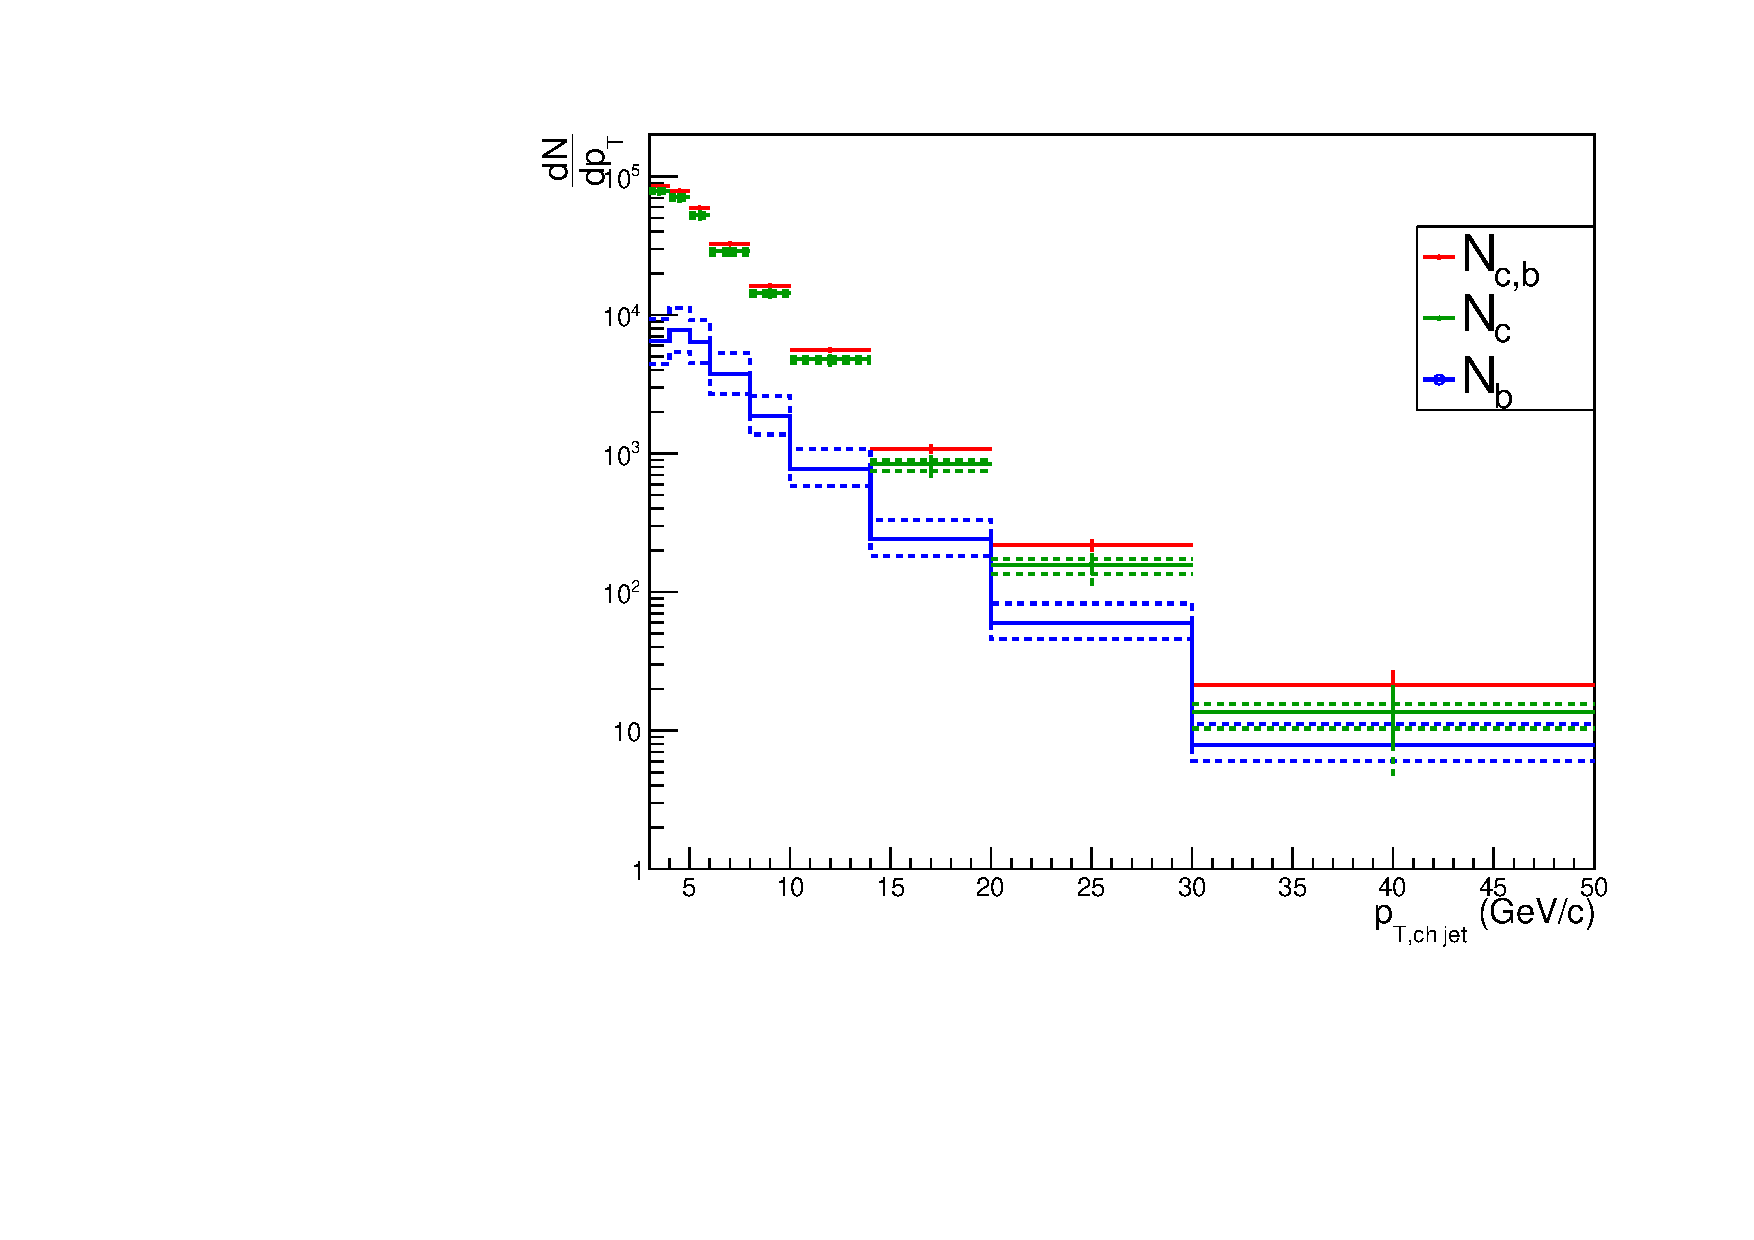
\includegraphics[width=\textwidth]{img/pPb/cSpectra5EX.pdf}}
\column{0.4\textwidth}
Analysis Steps
\vspace{5pt}
\small
\begin{easylist}[itemize]
@ Extraction of raw yield spectra with side-band subtraction method (same as in \pp\ analysis)
@ \textcolor{BrickRed}{Correction for reconstruction efficiency}
@ Subtraction of \textcolor{NavyBlue}{B feed-down}
@@ \textcolor{ForestGreen}{B feed-down corrected spectrum}
@ Presently working on: \textbf{unfolding for detector finite jet momentum resolution}
\end{easylist}
\end{columns}
\end{frame}

\subsection{Response Matrices}

\begin{frame}{Detector Resolution and Background Fluctuations}
\begin{columns}
\column{0.5\textwidth}
\centering	 
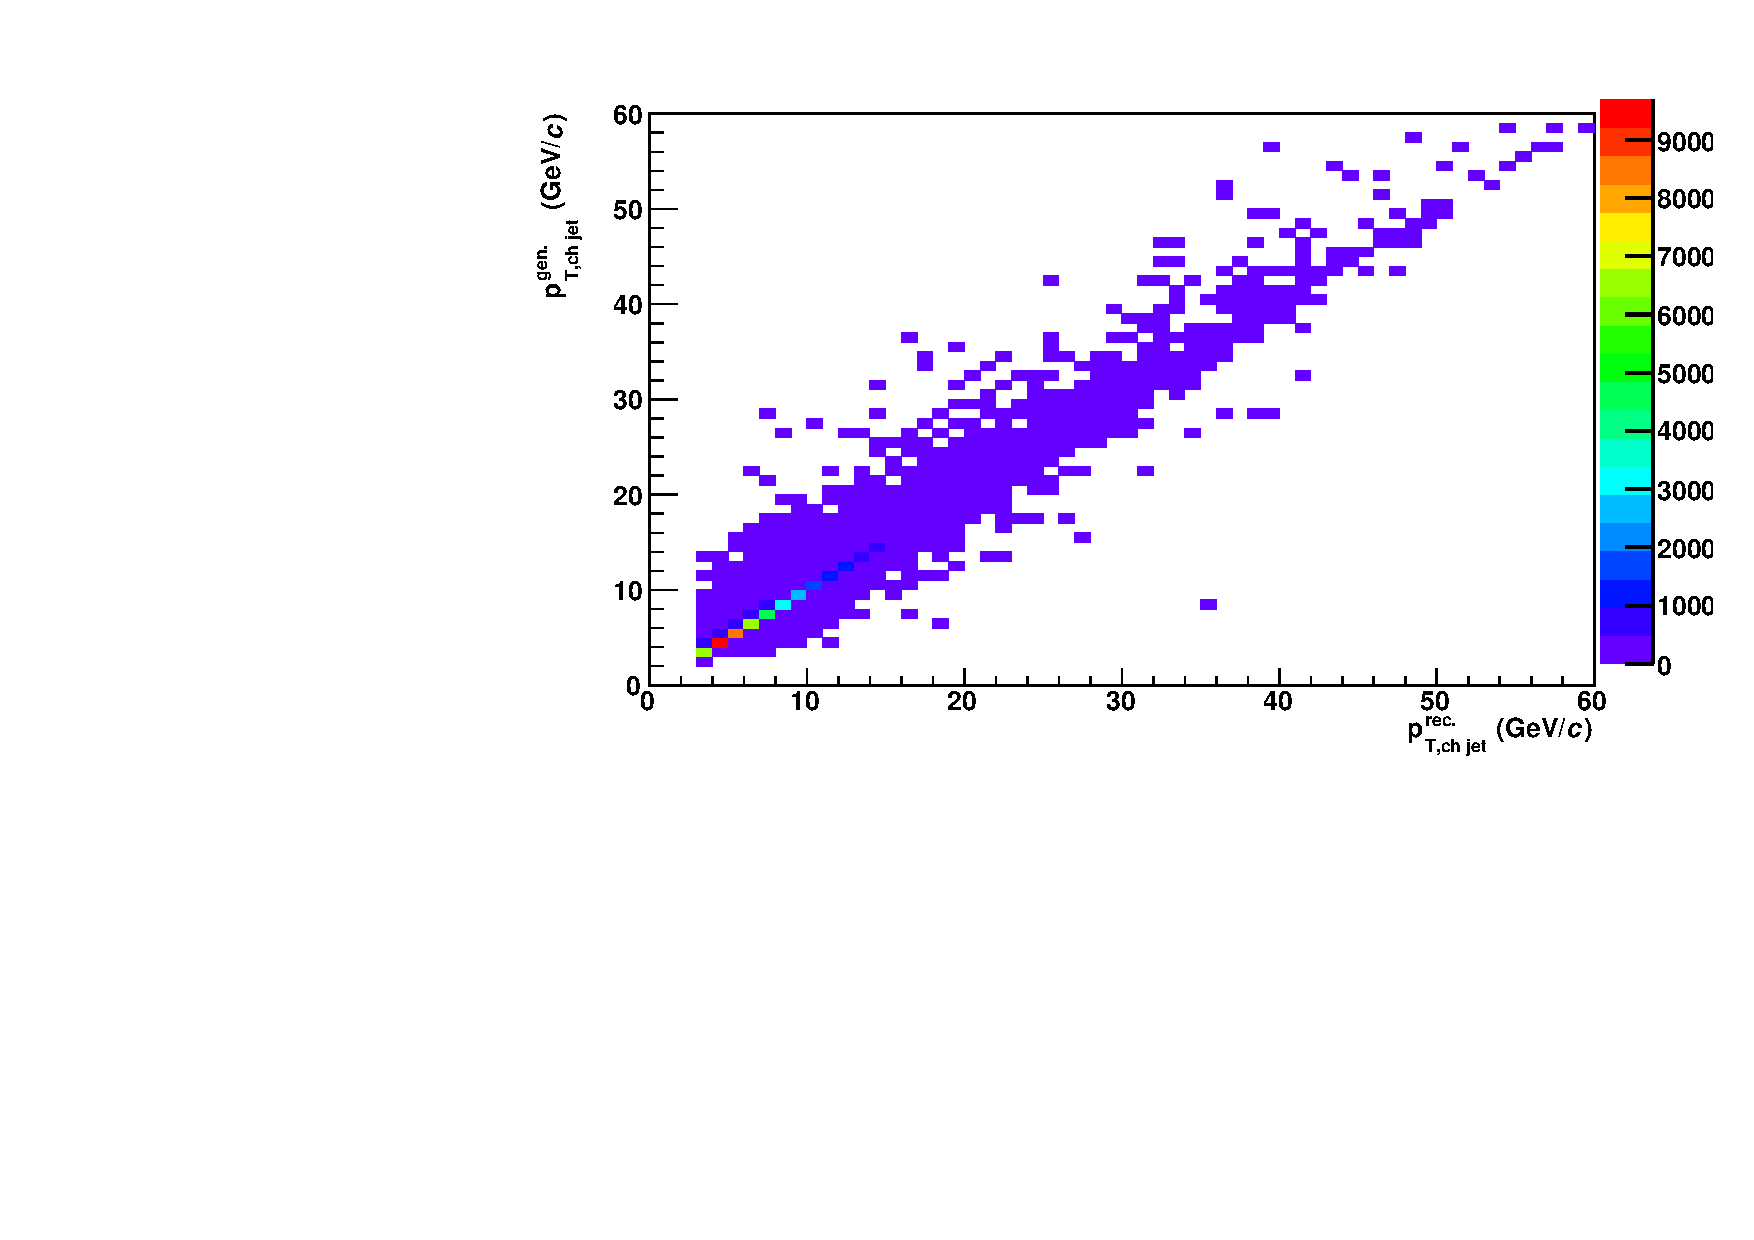
\includegraphics[width=\textwidth]{img/pPb/detMatrix.pdf}\\
\small
Detector response matrix for $3<\ptd<36$~\GeVc
\column{0.5\textwidth}
Random cones, excluding the leading jet
\centering
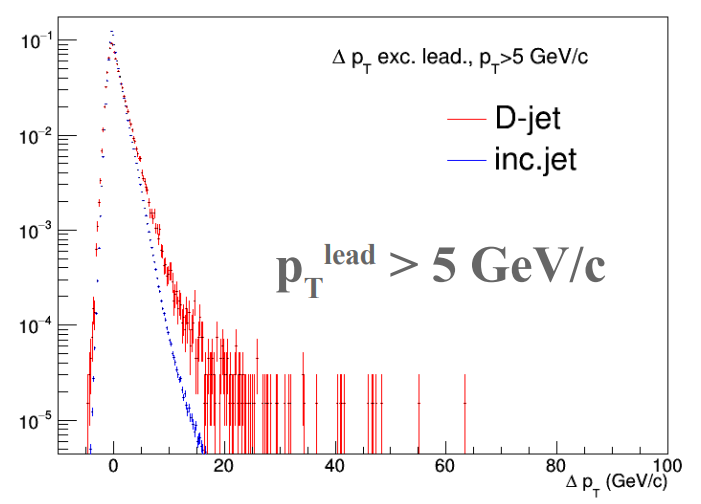
\includegraphics[width=0.8\textwidth]{img/pPb/delta_pT.png}\\
\footnotesize
\Dzero-jet candidate with
leading jet $\pt>$5~\GeVc\ required
\end{columns}
\end{frame}

\begin{frame}{Response matrices}
Generated jet \pt\ (vertical axis) vs Reconstructed jet \pt\ (horizontal axis)
\begin{columns}
\column{0.5\textwidth}
\centering
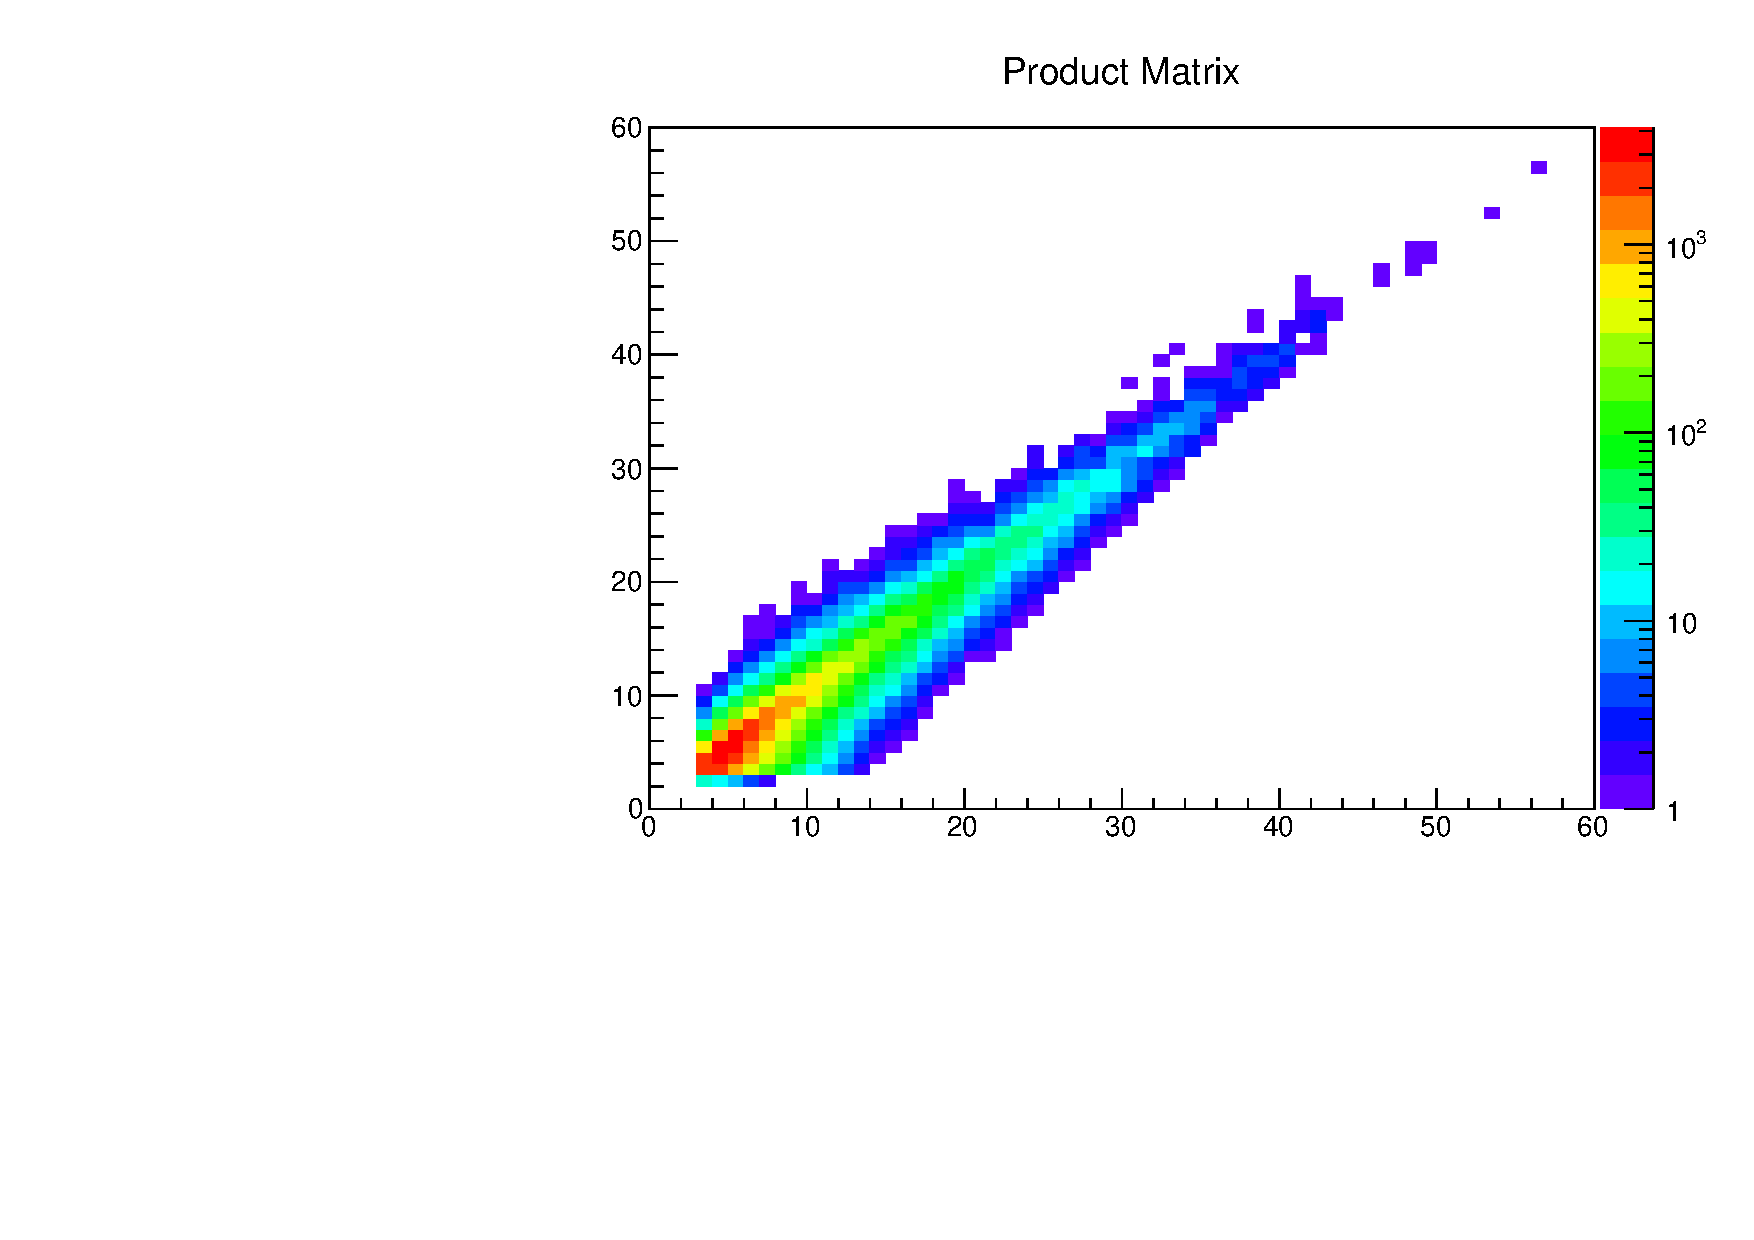
\includegraphics[width=0.9\textwidth]{img/pPb/productMatrix.pdf}\\
\small
Combined matrix: detector response $\times$ background fluctuations, \\
with $3<\ptd<36$~\GeVc
\column{0.5\textwidth}
\centering
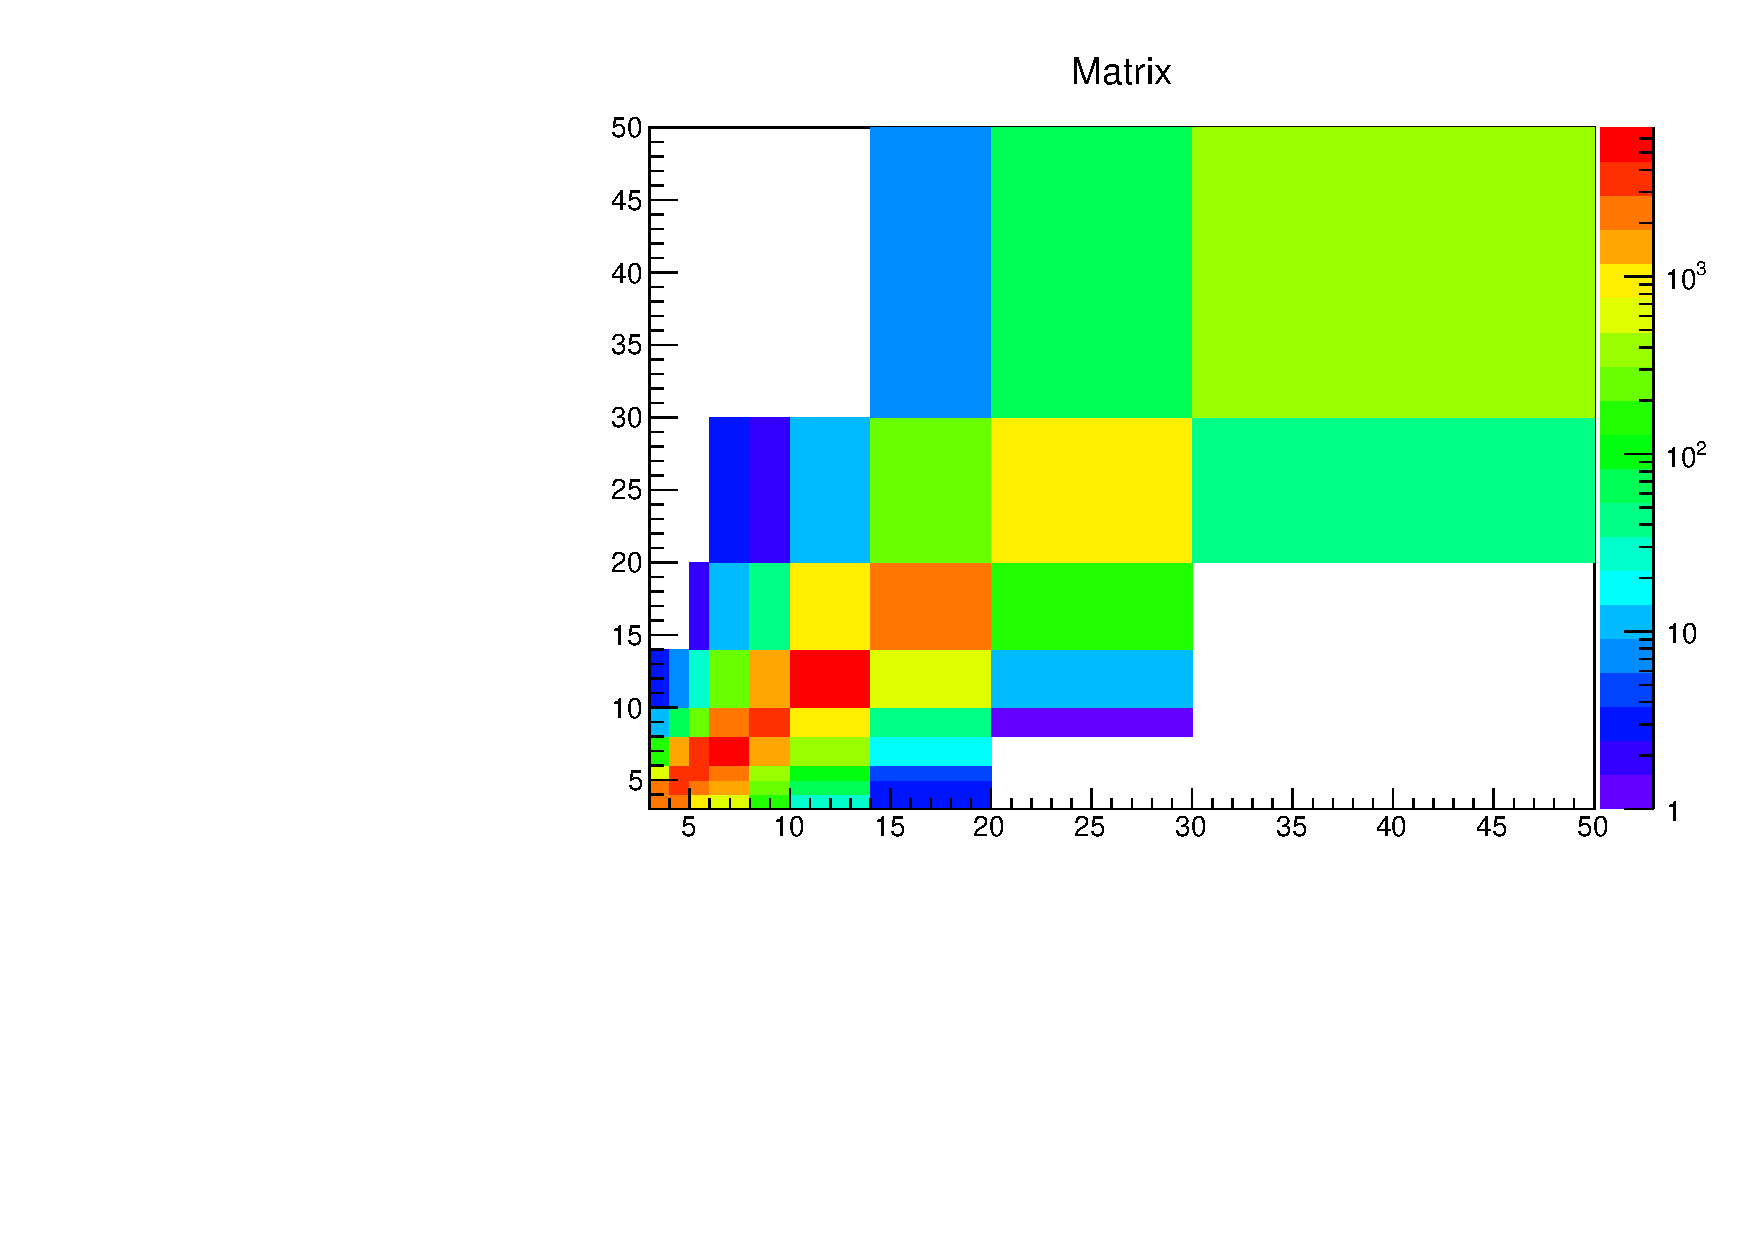
\includegraphics[width=0.9\textwidth]{img/pPb/productMatrixRebinned.pdf}\\
\small
Combined matrix re-binned to match the binning used for the measured spectrum
\end{columns}
\end{frame}

\subsection{Bayesian Unfolding}

\begin{frame}[fragile]{Bayes Unfolding}
\begin{columns}
\column{0.6\textwidth}
\centering
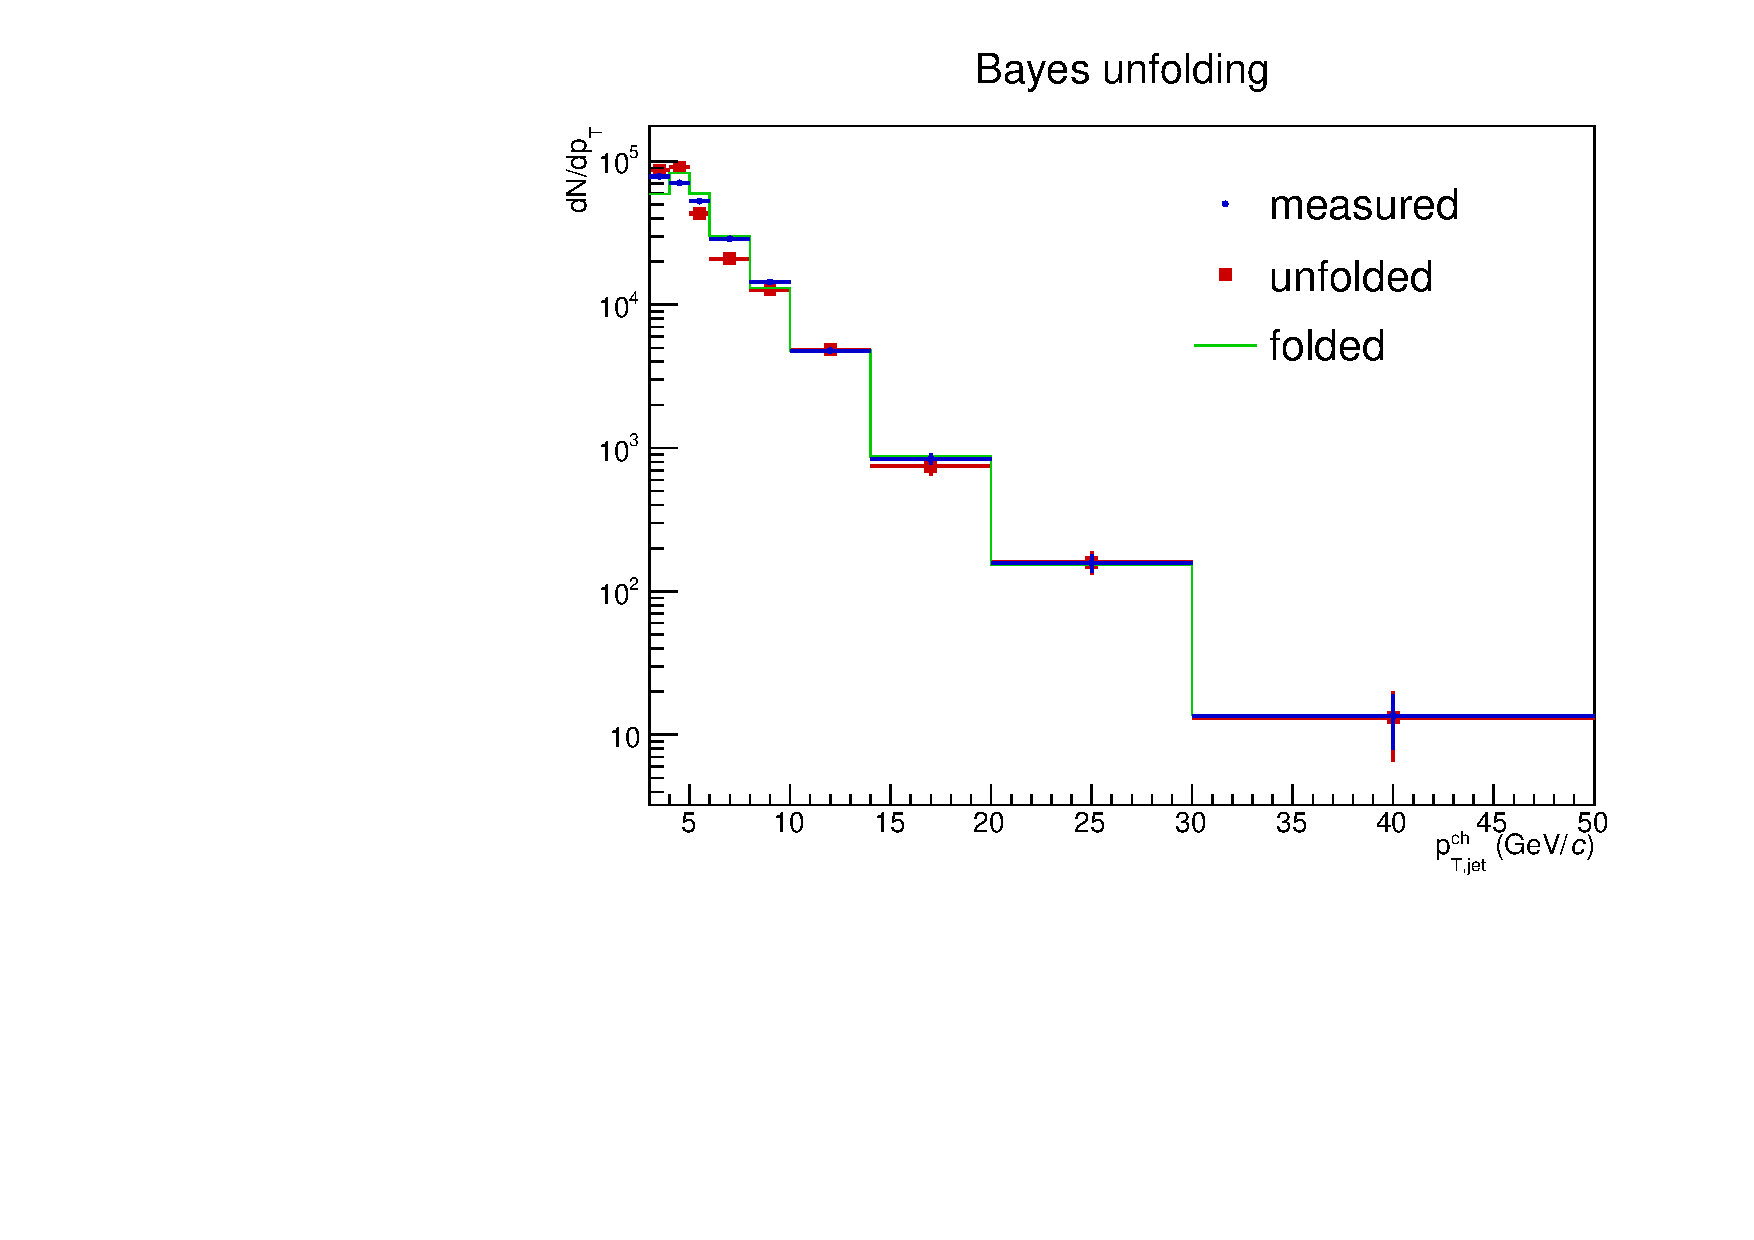
\includegraphics[width=\textwidth]{img/pPb/PythiaRM_Djet5Excl_bayes5_weight_3_50_3_50_UnfSpectrum.pdf}
\column{0.4\textwidth}
\begin{easylist}[itemize]
@ \textcolor{NavyBlue}{Measured spectrum}
@ \textcolor{BrickRed}{Bayes unfolded} spectrum
@@ Number of iterations: 5
@@ MC truth used as prior
@ \textcolor{ForestGreen}{Folded back} spectrum
\end{easylist}
\end{columns}
\end{frame}

\begin{frame}{Number of iterations}
\begin{columns}
\column{0.5\textwidth}
\centering
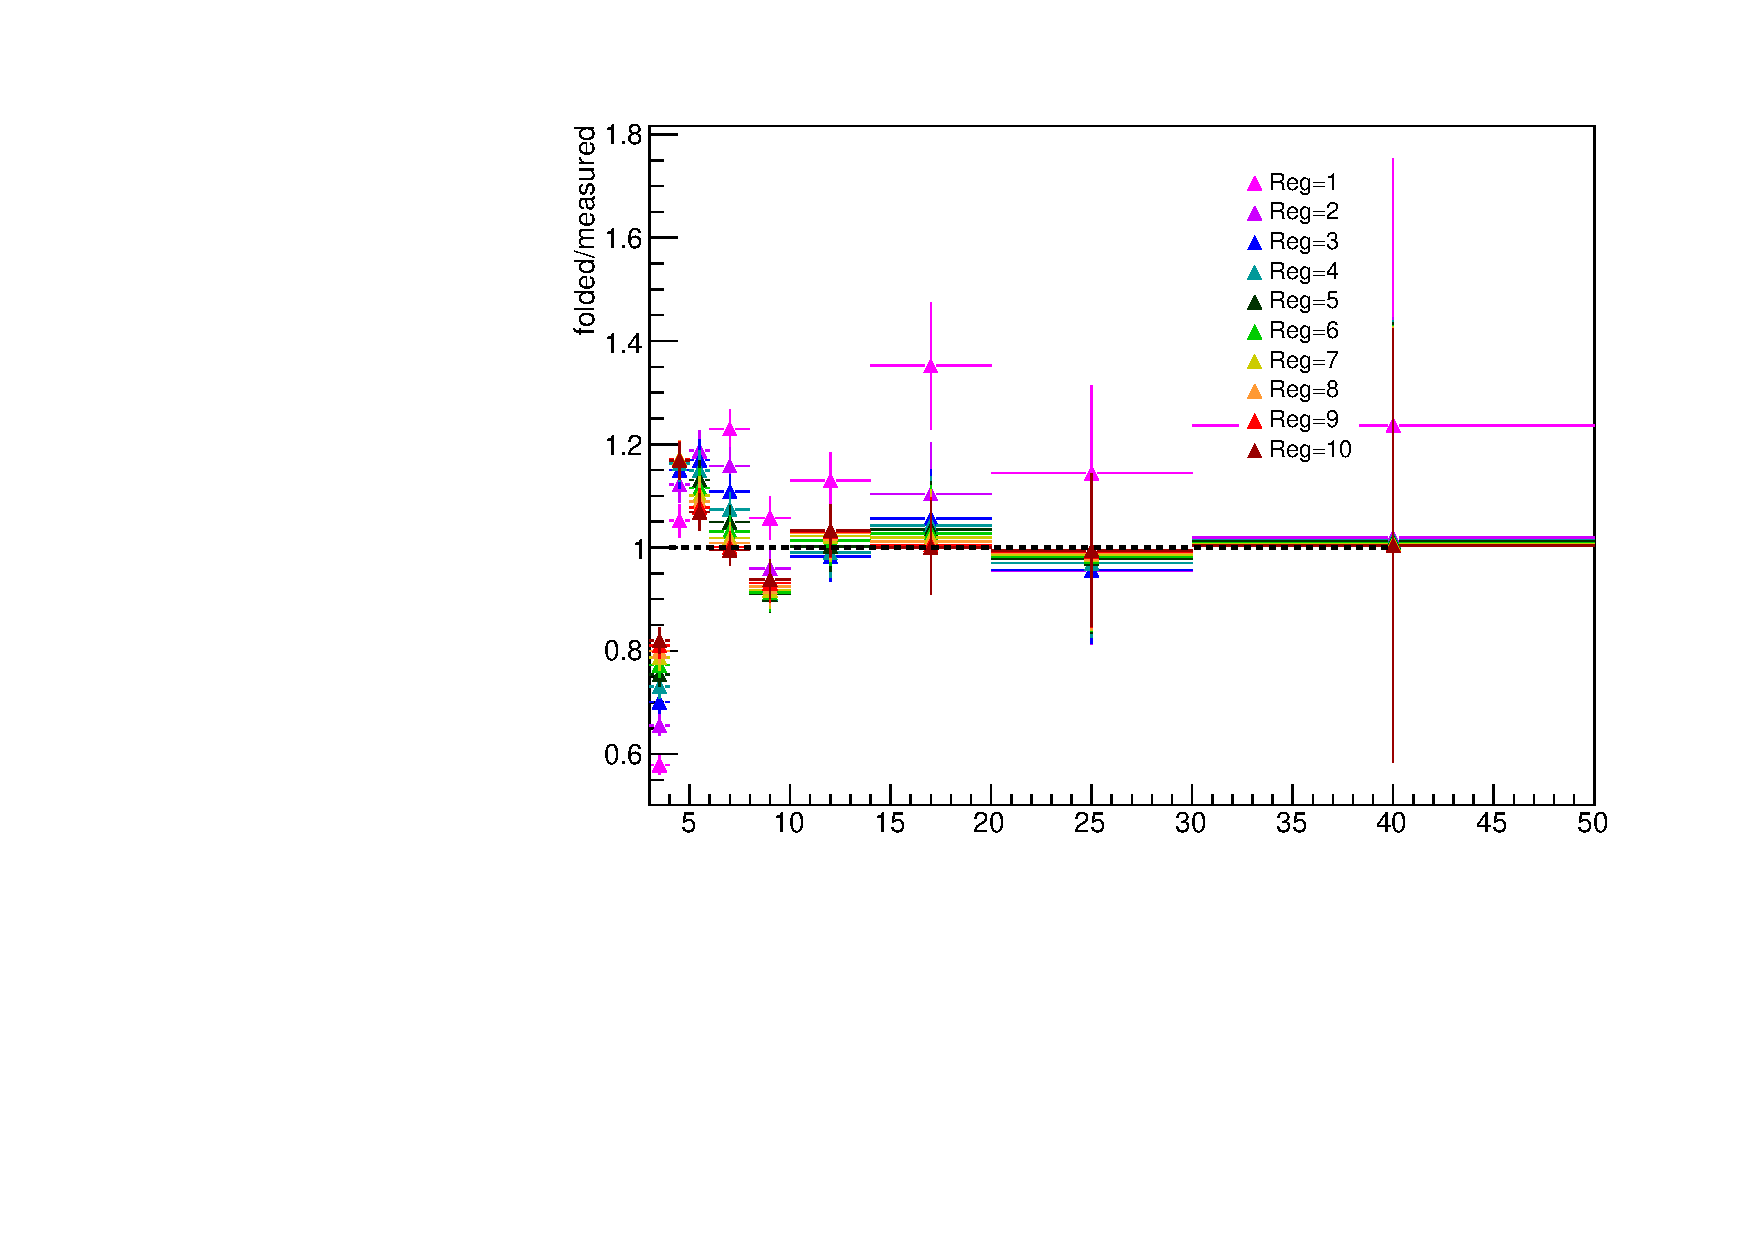
\includegraphics[width=\textwidth]{img/pPb/PythiaRM_Djet5Excl_bayes5_weight_3_50_3_50_foldedRatio.pdf}\\
\small
Re-folded spectra vs measured spectrum
\column{0.5\textwidth}
\centering
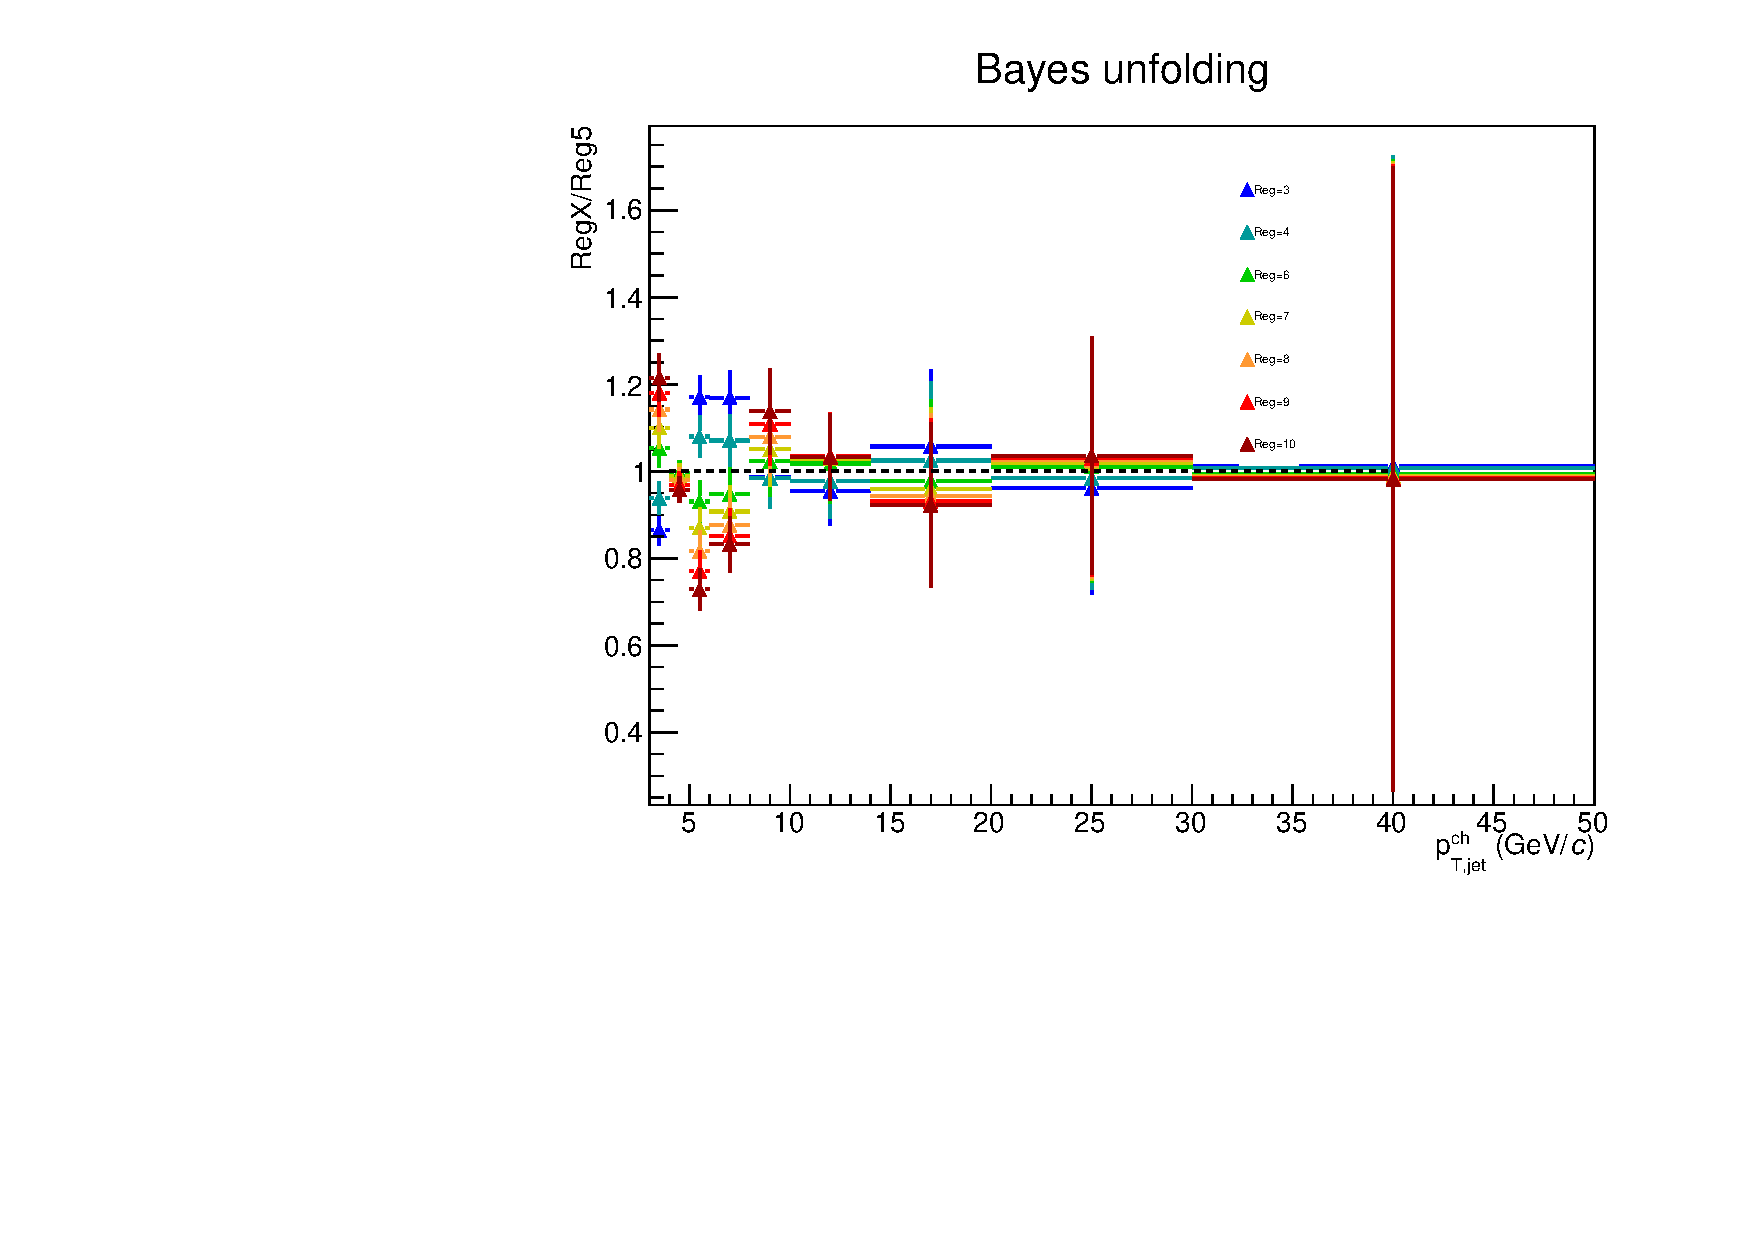
\includegraphics[width=\textwidth]{img/pPb/PythiaRM_Djet5Excl_bayes5_weight_3_50_3_50_unfRatio.pdf}\\
\small
Unfolded spectra ratio vs. default (5 iterations)
\end{columns}
\end{frame}

\begin{frame}{Background fluctuations and prior choice}
\begin{columns}[t]
\column{0.5\textwidth}
\centering
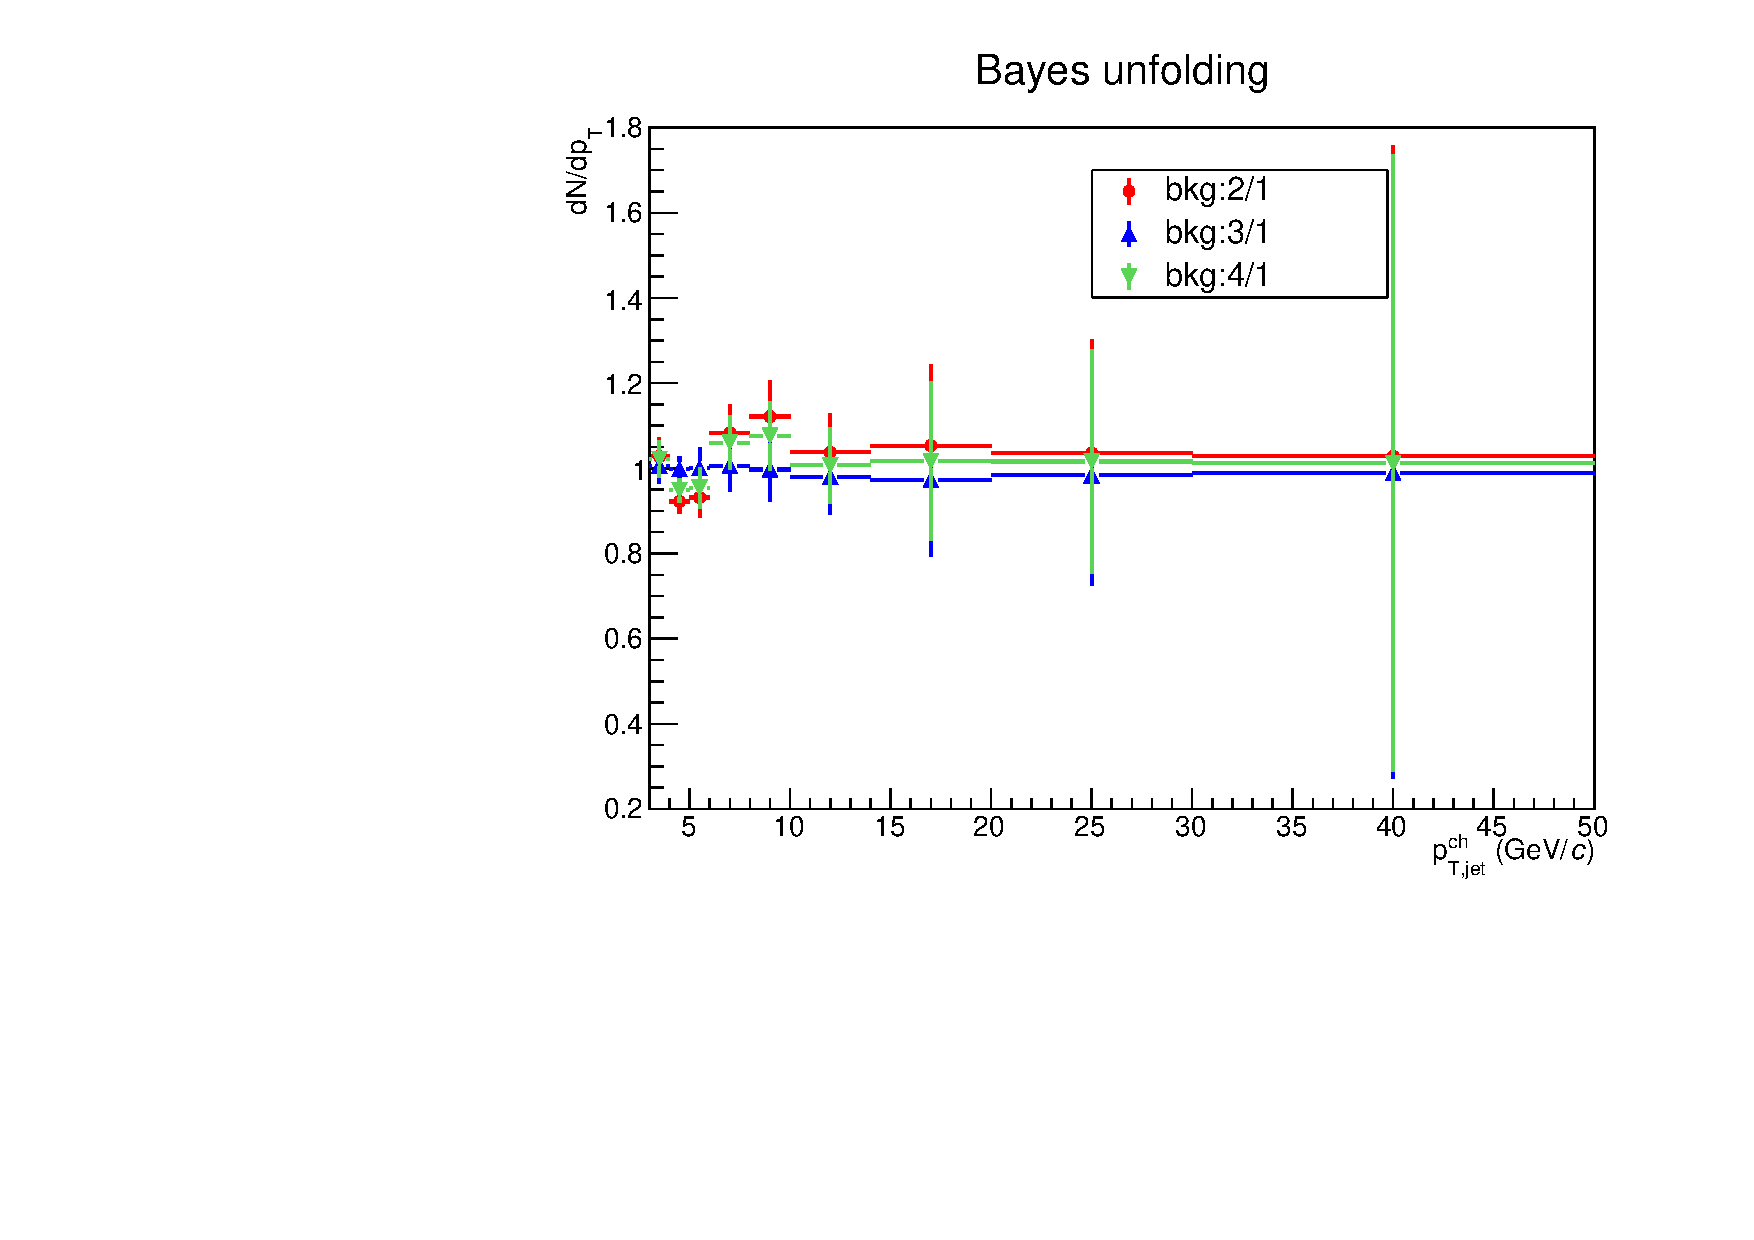
\includegraphics[width=0.75\textwidth]{img/pPb/3_36_step1_3_50_ratio_bkg.pdf}\\
\footnotesize
Different background fluctuations matrices:
\scriptsize
\begin{enumerate}
\item Leading \Dzero\ jet $\pt > 5$~\GeVc\ (default)
\item \textcolor{BrickRed}{Leading jet $\pt > 5$~\GeVc}
\item \textcolor{NavyBlue}{Leading \Dzero\ jet $\pt > 10$~\GeVc}
\item \textcolor{ForestGreen}{Leading jet $\pt > 10$~\GeVc}
\end{enumerate}
\column{0.5\textwidth}
\centering
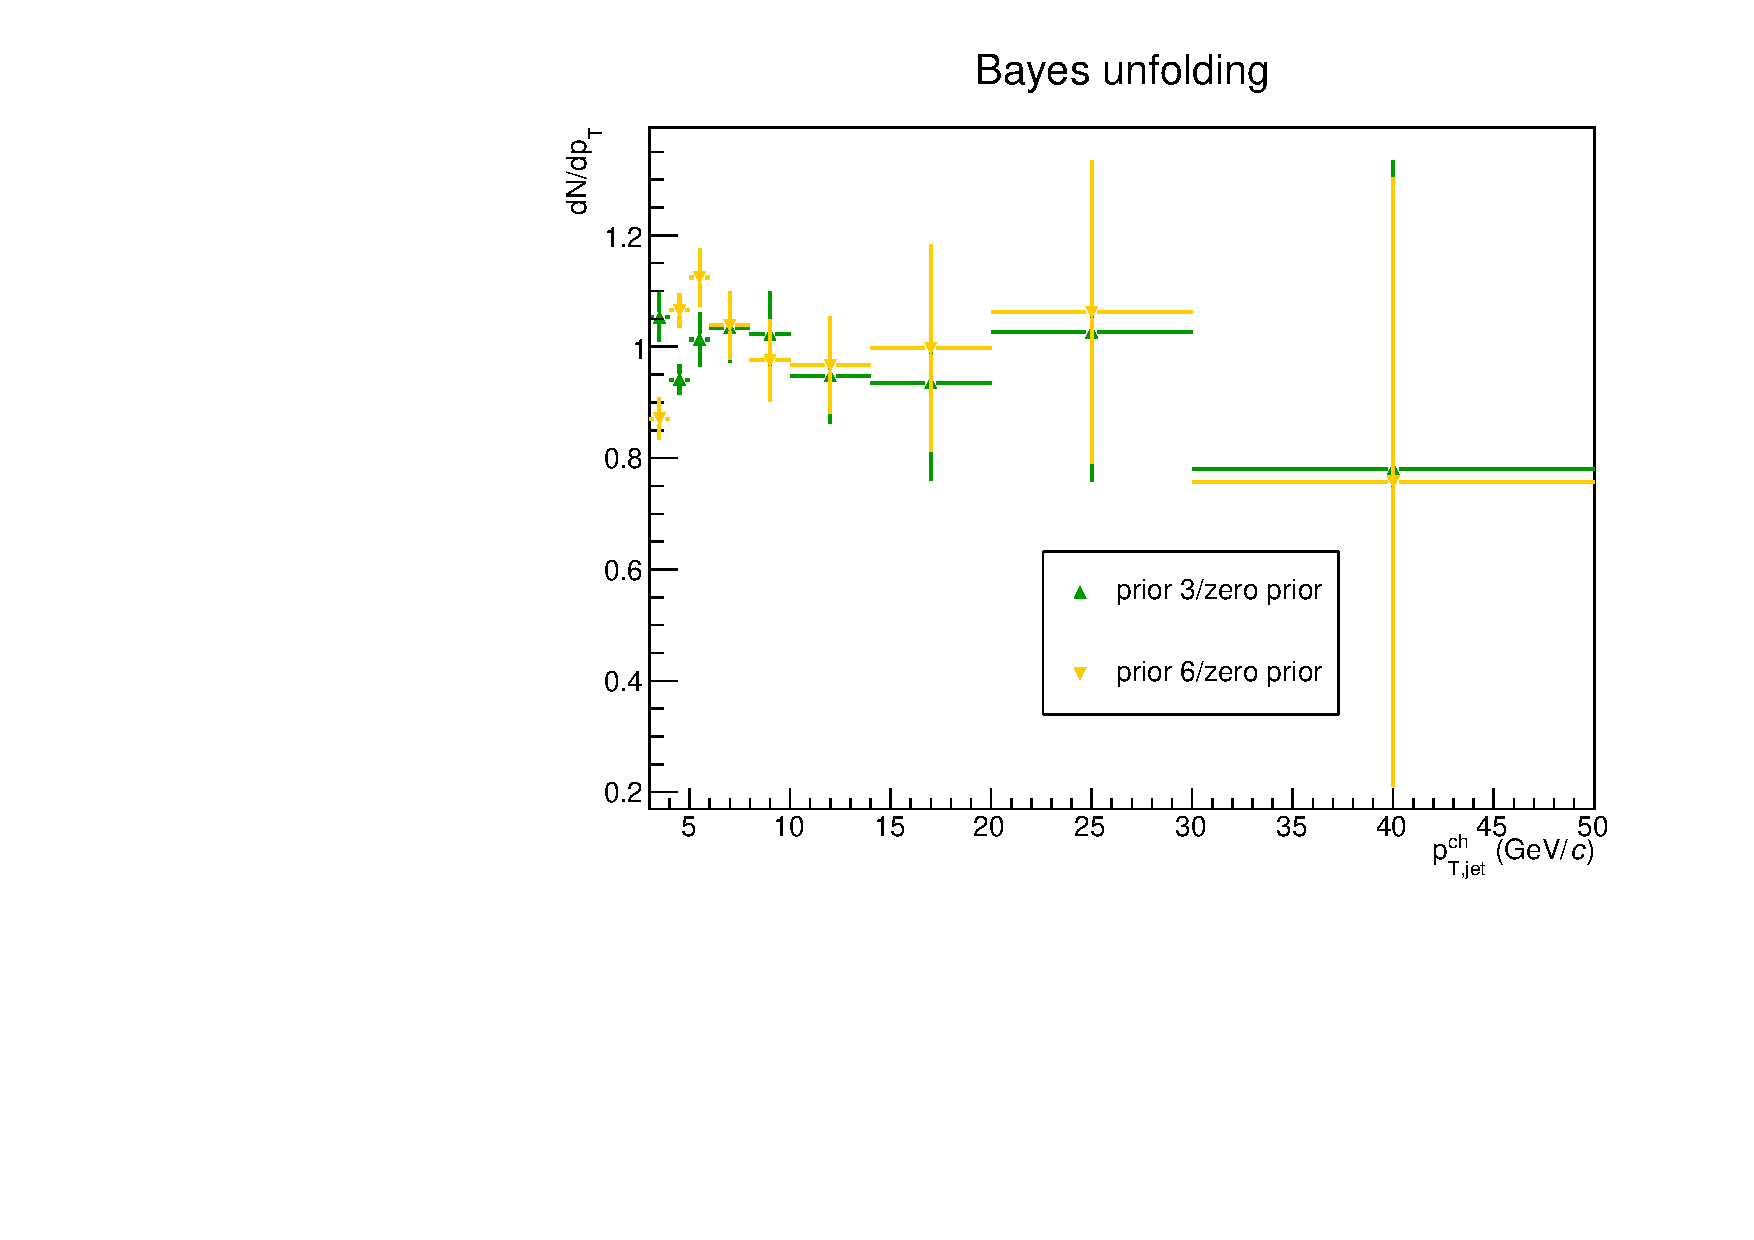
\includegraphics[width=0.75\textwidth]{img/pPb/priorRatio.pdf}\\
\footnotesize
Unfolded spectra ratio with different priors:\\
\scriptsize
\begin{itemize}
\item \textcolor{ForestGreen}{Prior 3}: $ax^{-3}e^{-18/x}$
\item \textcolor{YellowOrange}{Prior 6}: $ax^{-6}e^{-36/x}$
\end{itemize}
\end{columns}
\vspace{5pt}
\centering
\small
Small effect on the unfolded spectrum
\end{frame}

\subsection{SVD Unfolding}

\begin{frame}{SVD Unfolding}
\begin{columns}
\column{0.5\textwidth}
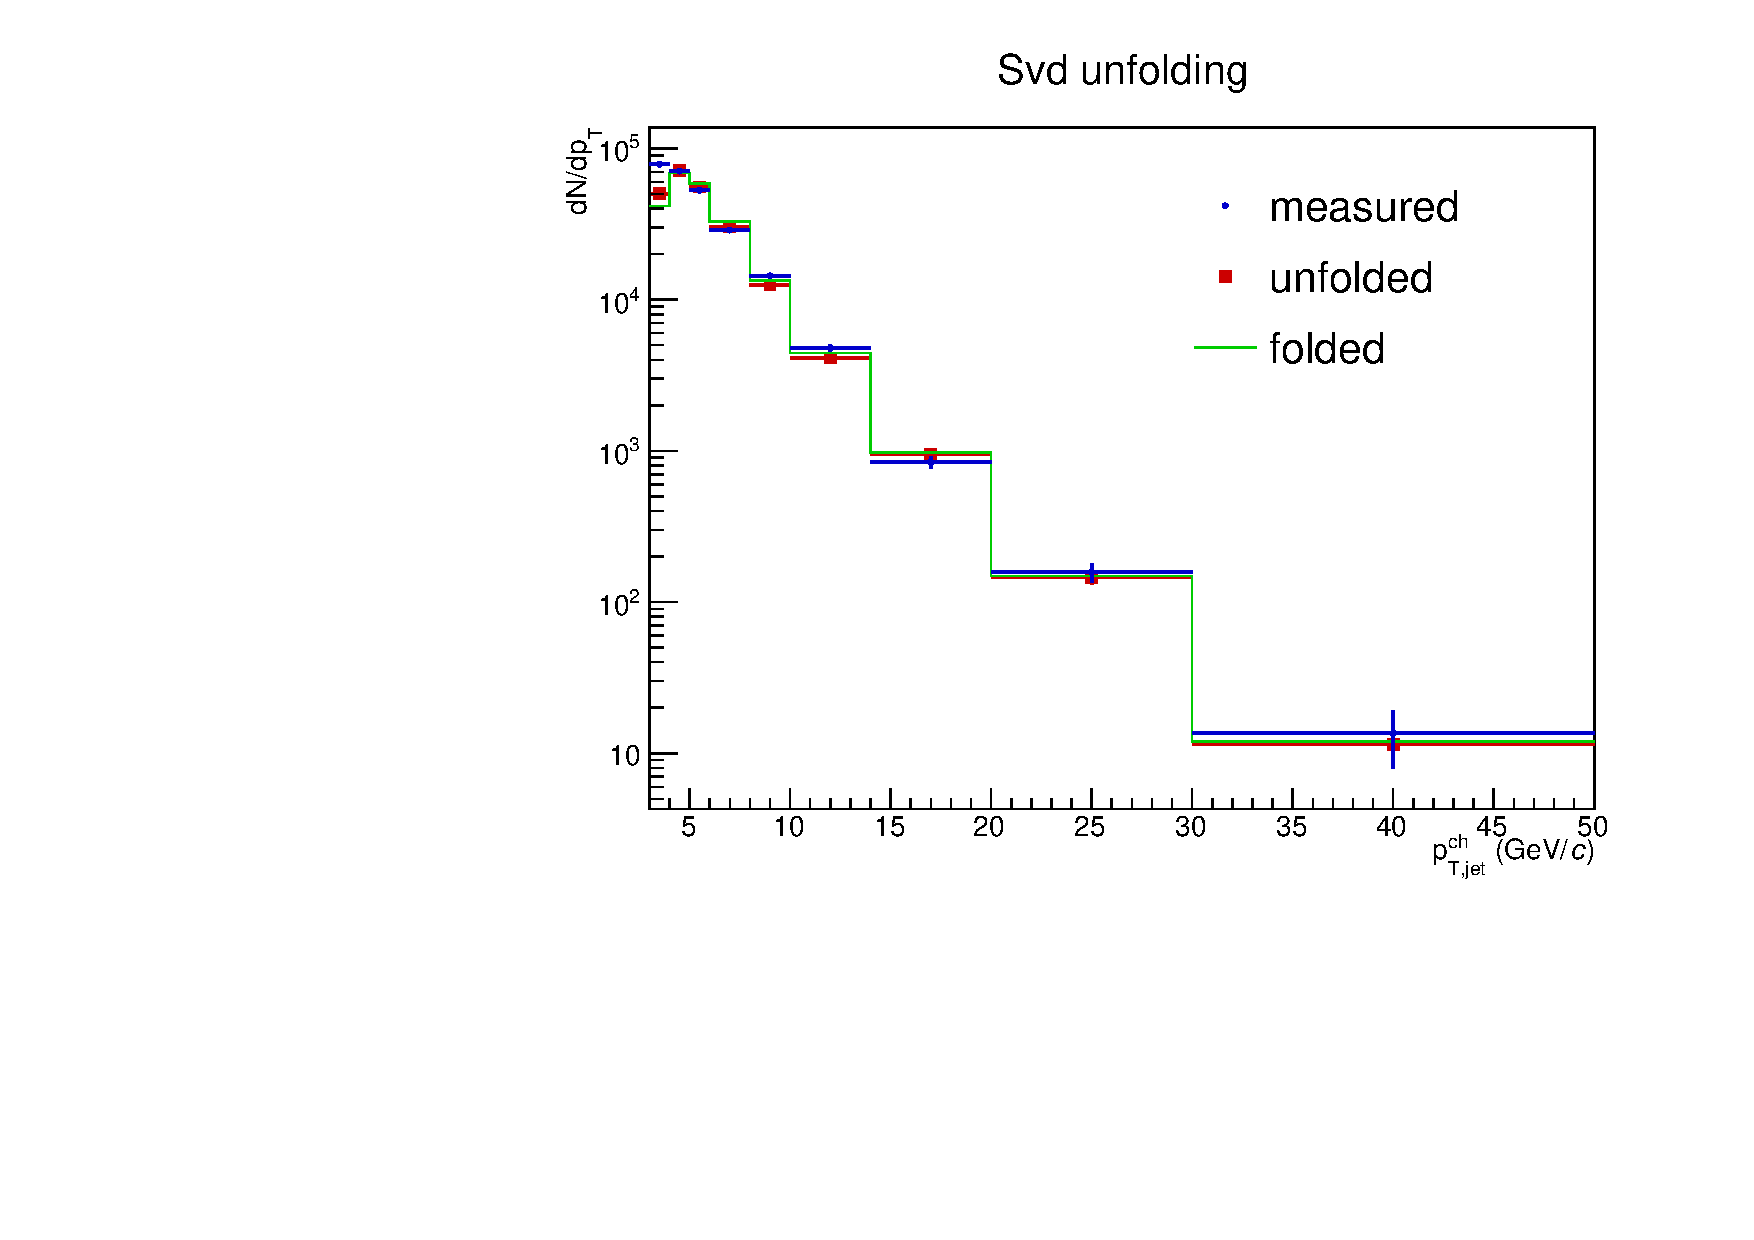
\includegraphics[width=\textwidth]{img/pPb/SvdReg3.pdf}\\
\small
SVD unfolding: regularisation param=3
\column{0.5\textwidth}
\centering
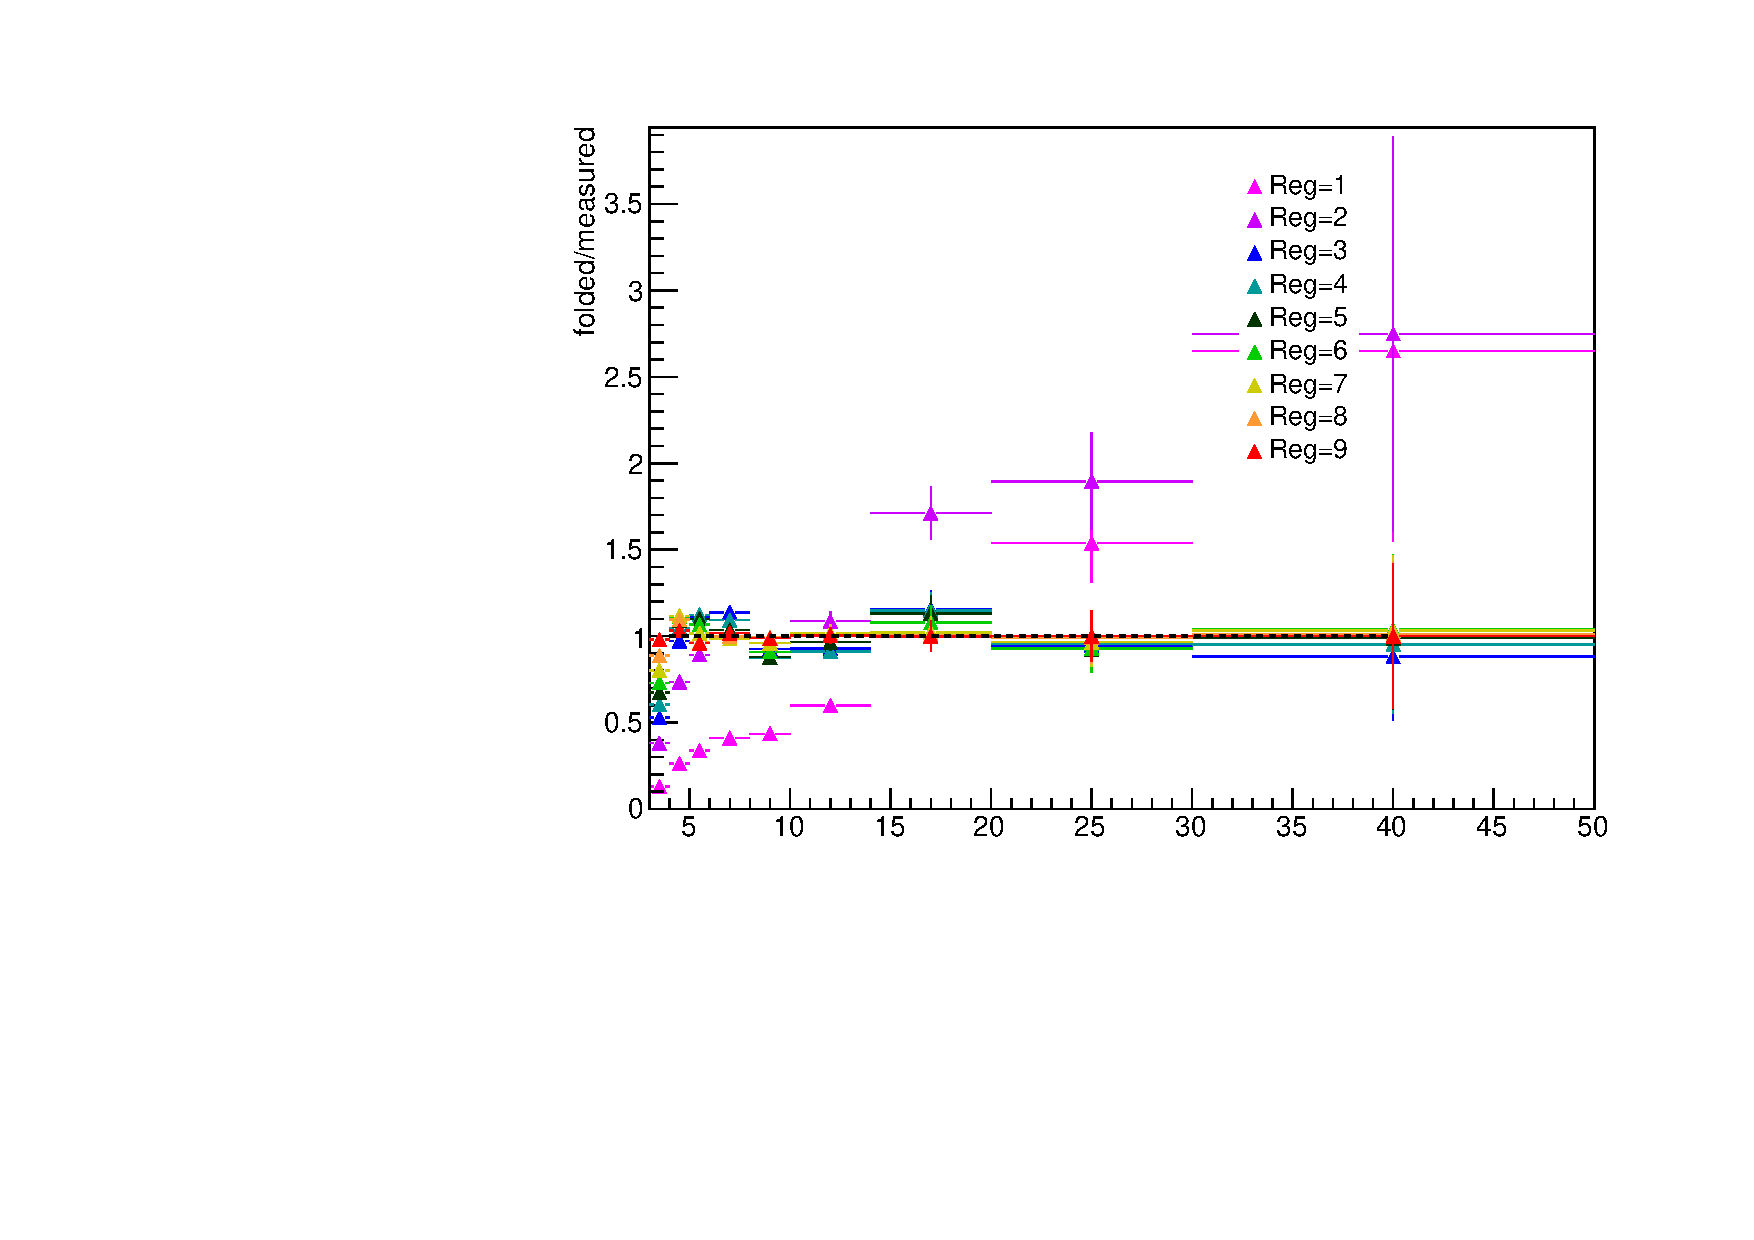
\includegraphics[width=\textwidth]{img/pPb/SvdFoldMeas.pdf}\\
\small
SVD: Folded spectra with diff regularisation parameters vs measured spectrum
\end{columns}
\end{frame}

\begin{frame}{SVD regularization}
\begin{columns}
\column{0.5\textwidth}
\centering
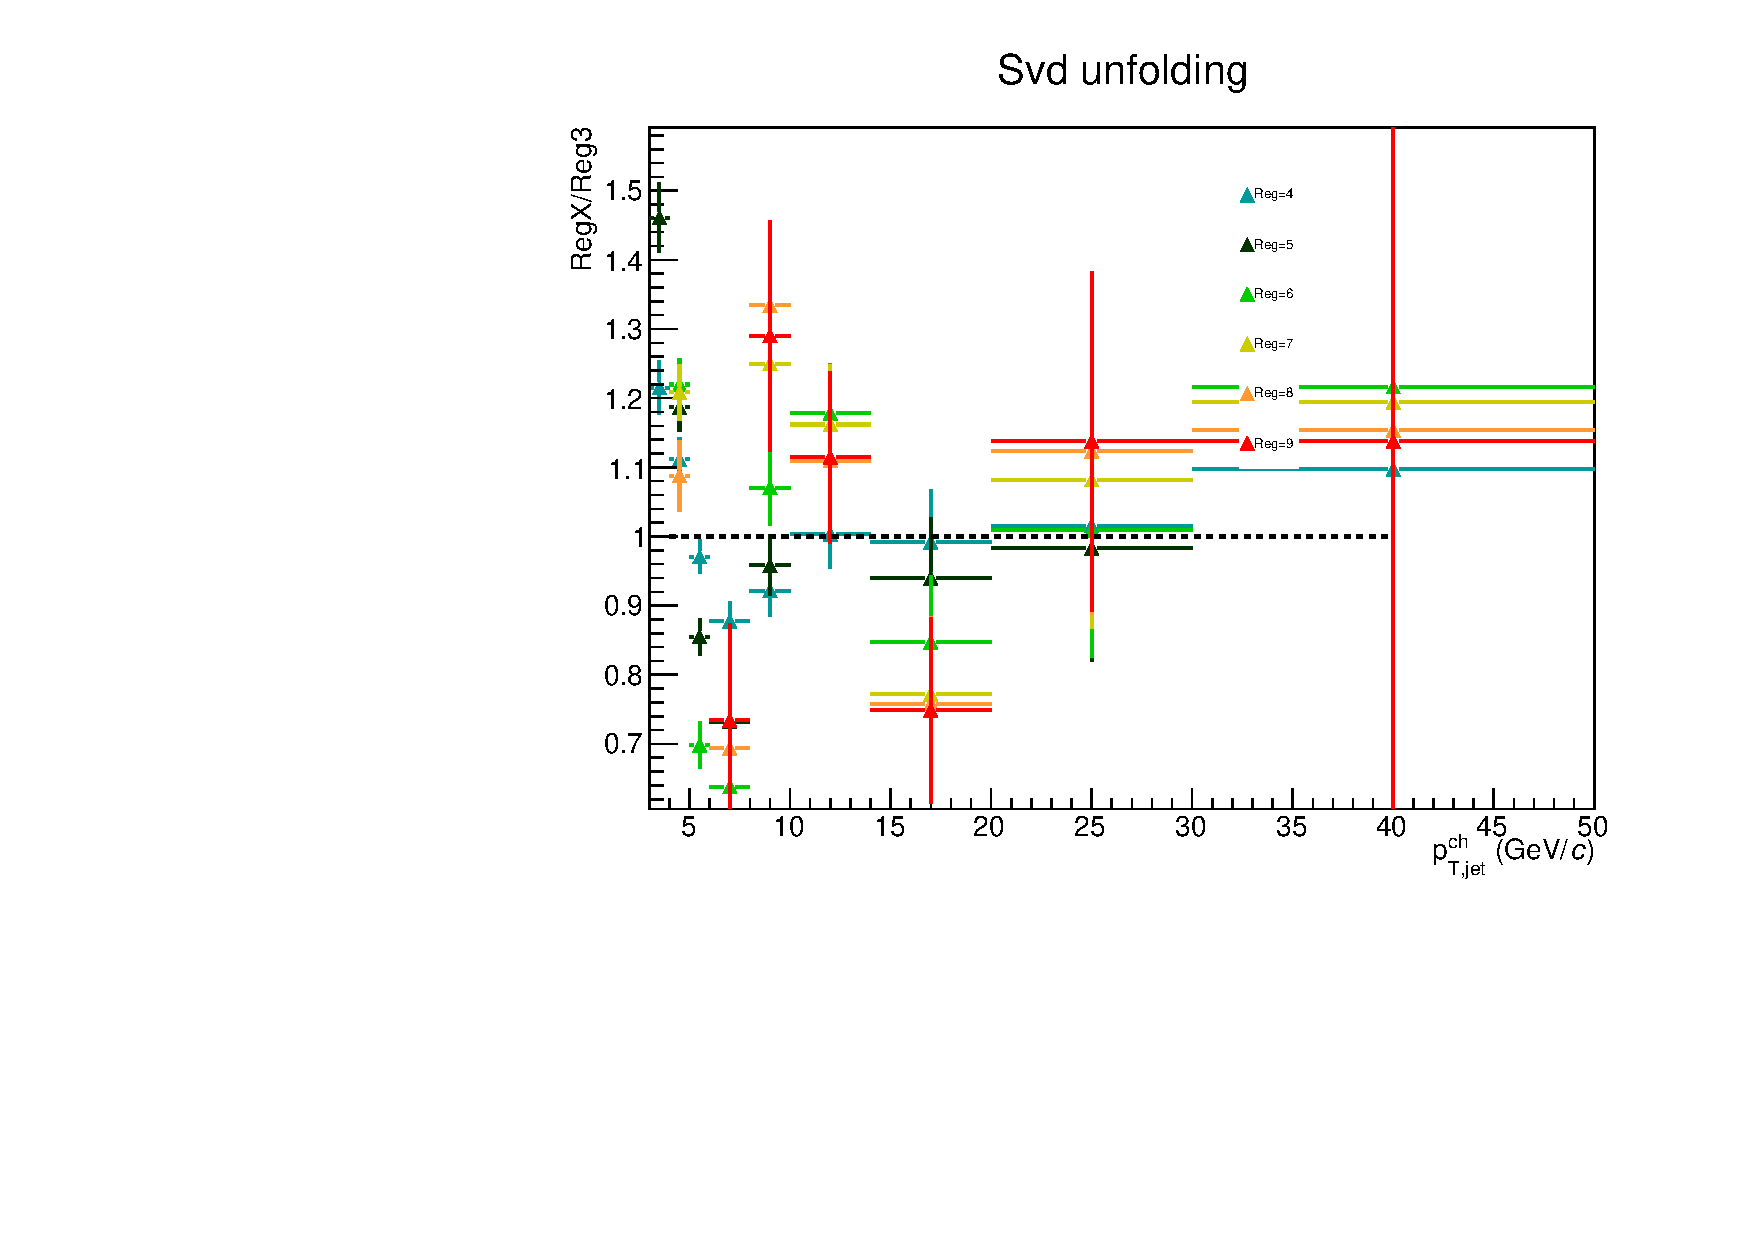
\includegraphics[width=0.95\textwidth]{img/pPb/SvdEvolutionRatio.pdf}\\
\small
Different regularizations vs $k=3$
\column{0.5\textwidth}
\centering
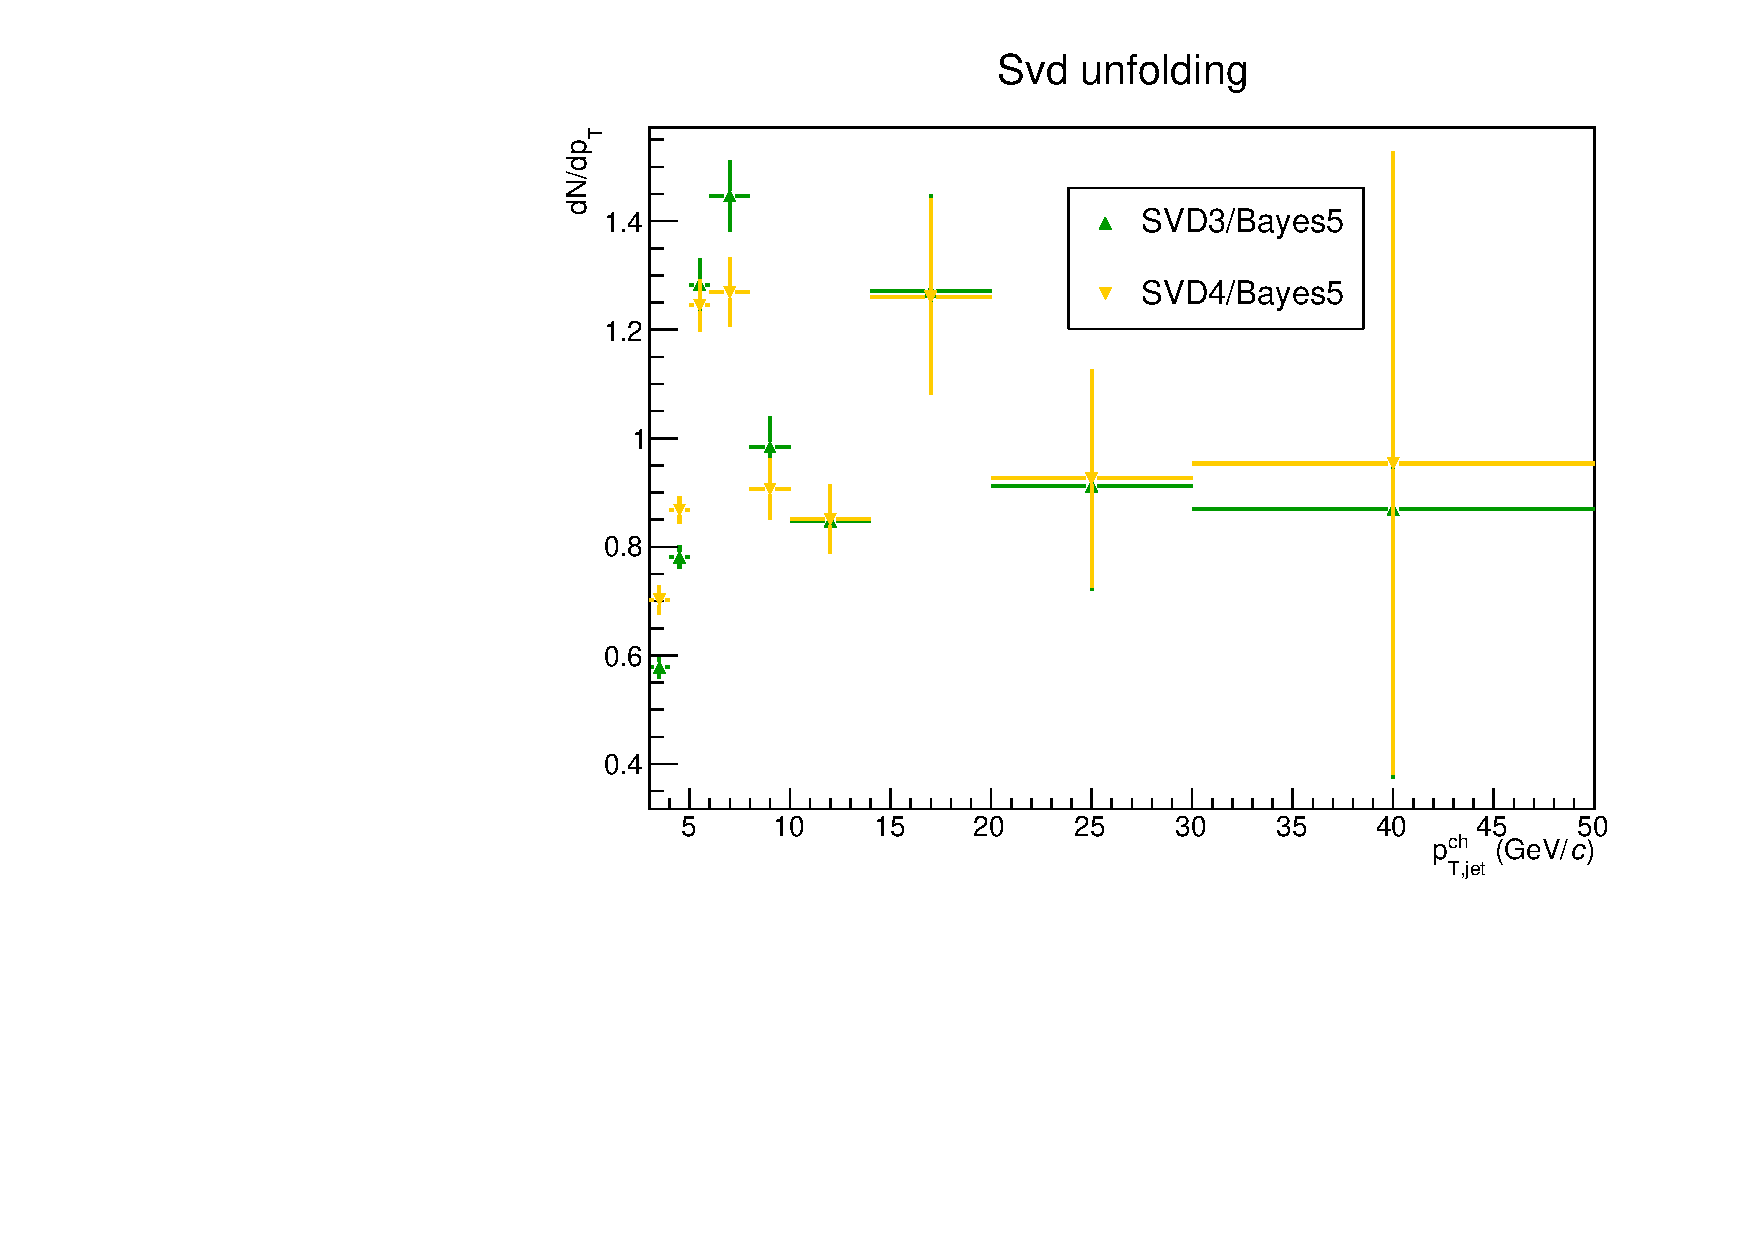
\includegraphics[width=0.95\textwidth]{img/pPb/SvdBayesRatio.pdf}\\
\small
$k=3, 4$ vs Bayes unfolding with reg$=5$
\end{columns}
\small
\centering
\vspace{10pt}
Biggest deviation is observed in the bins $5<\ptchjet<7$~\GeVc
\end{frame}

\section{Conclusions}

\begin{frame}[fragile]{Conclusions}
\footnotesize
\begin{easylist}[itemize]
@ \pp\ collisions at $\s=7$~TeV
@@ Minor updates for the \textbf{jet cross section} (preliminary approved for QM17)
@@ Distribution of the \textbf{jet momentum fraction carried by the \Dzero} \alert{[NEW]}
@@ Paper proposal approved at PF on 17/01/2018: \url{https://indico.cern.ch/event/694977/} 
@@ To do: use EvtGen as default decayer for the B feed-down subtraction (in progress)
@@ To do: more theoretical comparisons (POWHGE LO, PYTHIA8, HERWIG, ...)
@@ To do: re-weight D-tagged jets in RM simulation to match the measured jet \pt\ spectrum
@ \pPb\ collisions at $\s=5.02$~TeV
@@ Analysis being done with \Dzero\ (preliminary already approved for \Dstar\ jets)
@@ Raw yield extraction, efficiency correction and B feed-down correction $\rightarrow$ \textbf{done}
@@ Working on unfolding: need to check stability, understand differences between SVD and Bayesian, try also bin-by-bin correction
\end{easylist}
\end{frame}

\appendix

\section{Extra Slides}

\begin{frame}{Useful links (\pp\ analysis)}
JIRA ticket: \url{https://alice.its.cern.ch/jira/browse/PWGHF-108}\\
\vspace{10pt}
Analysis code: \url{https://github.com/aiola/alice-yale-hfjet}\\
\vspace{10pt}
Analysis note and paper draft repository: \url{https://gitlab.cern.ch/saiola/PaperD0JetsPP2010}\\
\vspace{10pt}
Analysis note on aliceinfo: \url{https://aliceinfo.cern.ch/Notes/node/587}
\end{frame}

\subsection{Paper Proposal}

\begin{frame}[fragile]{Paper Proposal}
\vspace{-10pt}
\begin{center}
``Measurement of the \pt-differential cross-section and fragmentation function of \Dzero-tagged charged jets in \pp\ collisions at $\s=7$~TeV with ALICE''
\end{center}
\scriptsize
\begin{easylist}[itemize]
@ Target journal: JHEP
@ PC: Salvatore Aiola (chair), Barbara Trzeciak, Antonio Silva, Andrea Rossi
@ ARC (for the preliminary approved in January 2017): Leticia Conqueiro, Jeremy Wilkinson, Yasser Morales
\only<1> {
@ Outline of the paper
@@ \textbf{Introduction}: Physics case for charm jets
@@ \textbf{ALICE}: Short description of the detector, particularly the ITS, TPC, TOF, V0
@@ \textbf{Data and Monte Carlo Samples}: Description of the data and MC sample used for the analysis
@@ \textbf{D-Tagged Jet Reconstruction}: Description of the analysis procedure (D-meson and jet reconstruction)
@@ \textbf{Raw Signal Extraction}: Invariant mass fits, raw yields, efficiency, B feed-down
@@ \textbf{Unfolding}: Discussion of the resolution and detector response unfolding
@@ \textbf{Systematic Uncertainties}: Discussion of the systematic uncertainties
@@ \textbf{Results}: Cross section and momentum fraction distributions, comparison with models
@@ \textbf{Conclusions}: Wrapping up and outlook
}
\only<2>{
@ Figures
@@ Reconstruction efficiency (2 figures)
@@ Invariant mass fit and side-band subtraction (2 figures)
@@ Raw B feed-down fraction (3 figures)
@@ Jet momentum resolution
@@ Momentum fraction resolution
@@ Uncertainties (3 figures)
@@ Jet cross section
@@ Distribution of the momentum fraction carried by the \Dzero\ (2 figures)
}
\end{easylist}
\end{frame}

\begin{frame}{Cross Section and Momentum Fraction Distribution}
\begin{columns}
\column{0.33\textwidth}
\centering
\footnotesize
Momentum Fraction Distribution: $5<\ptchjet<15$~\GeVc\\
\begin{overpic}[width=\textwidth, trim=0 0 0 0, clip]{img/paper_figures/JetZSpectrum_JetPt_5_15_Paper}
\end{overpic}
\column{0.33\textwidth}
\centering
\footnotesize
Momentum Fraction Distribution: $15<\ptchjet<30$~\GeVc\\
\begin{overpic}[width=\textwidth, trim=0 0 0 0, clip]{img/paper_figures/JetZSpectrum_JetPt_15_30_Paper}
\end{overpic}
\column{0.34\textwidth}
\footnotesize
Jet \pt\ cross section\\
\begin{overpic}[width=\textwidth, trim=0 0 0 0, clip]{img/paper_figures/D0JetCrossSection_Paper}
\end{overpic}
\end{columns}
\end{frame}

\begin{frame}{Side-Band Inv. Mass Analysis (Jet \pt\ Spectrum)}
\centering
\begin{overpic}[width=.7\textwidth, trim=0 0 0 0, clip]{img/paper_figures/SideBandInvMass_Paper}
\end{overpic}
\end{frame}

\begin{frame}{Side-Band Inv. Mass Analysis (\zpar\ Distributions)}
\centering
\begin{overpic}[width=.7\textwidth, trim=0 0 0 0, clip]{img/paper_figures/SideBandInvMass_Z_Paper}
\end{overpic}
\end{frame}

\begin{frame}{Reconstruction Efficiency}
\begin{columns}
\column{0.5\textwidth}
\begin{overpic}[width=\textwidth, trim=0 0 0 0, clip]{img/paper_figures/Efficiency_Paper}
\end{overpic}
\column{0.5\textwidth}
\begin{overpic}[width=\textwidth, trim=0 0 0 0, clip]{img/paper_figures/EfficiencyVsJetPt_Paper}
\end{overpic}
\end{columns}
\end{frame}

\begin{frame}{B Feed-Down}
\begin{columns}
\column{0.5\textwidth}
\centering
\footnotesize
Momentum Fraction Distribution\\
\begin{overpic}[width=\textwidth, trim=0 0 0 0, clip]{img/paper_figures/BFeedDown_JetZSpectrum_Paper}
\end{overpic}
\column{0.5\textwidth}
\centering
\footnotesize
Jet \pt\ cross section\\
\begin{overpic}[width=\textwidth, trim=0 0 0 0, clip]{img/paper_figures/BFeedDown_JetPtSpectrum_DPt_30_Paper}
\end{overpic}
\end{columns}
\end{frame}

\begin{frame}{Detector Resolution}
\begin{columns}
\column{0.5\textwidth}
\centering
\footnotesize
Momentum Fraction Distribution\\
\begin{overpic}[width=\textwidth, trim=0 0 0 0, clip]{img/paper_figures/ResolutionVsZ_Paper}
\end{overpic}
\column{0.5\textwidth}
\centering
\footnotesize
Jet \pt\ cross section\\
\begin{overpic}[width=\textwidth, trim=0 0 0 0, clip]{img/paper_figures/ResolutionVsJetPt_Paper}
\end{overpic}
\end{columns}
\end{frame}

\subsection{\pp\ collisions: uncertainties}

\begin{frame}{Uncertainty Summary: \ptchjet\ spectrum, $\ptd>3$~\GeVc}
\footnotesize
\begin{table}
\begin{tabular}{lrrrrrr}
Source & \multicolumn{6}{c}{Uncertainty (\%)} \\ \hline
\ptchjet\ (\GeVc) & 5 - 6 & 6 - 8 & 8 - 10 & 10 - 14 & 14 - 20 & 20 - 30\\ \hline
Tracking Eff. (Jet Energy Scale) & 0 & 1 & 2 & 3 & 4 & 4\\
Raw Yield Extraction & 4 & 5 & 5 & 5 & 11 & 15\\
B Feed-Down & 6 & 6 & 7 & 9 & 14 & 16\\
Unfolding & 5 & 5 & 5 & 5 & 5 & 5\\
Selection Cuts & 5 & 5 & 5 & 5 & 5 & 5\\
Tracking Eff. (D-Meson) & 4 & 4 & 4 & 4 & 4 & 4\\
\hline
Normalization (luminosity and BR) & \multicolumn{6}{c}{3.6} \\
\hline
Total Systematic Uncertainty & 11.5 & 11.9 & 12.5 & 13.9 & 20.3 & 24.0\\
\hline
Statistical & 10.0 & 9.0 & 12.3 & 15.9 & 23.7 & 64.1\\
\hline
Total Uncertainty & 15.2 & 14.9 & 17.6 & 21.2 & 31.2 & 68.5\\
  \end{tabular}
\end{table}
\end{frame}

\begin{frame}{Uncertainty Summary: \zpar\ spectrum, $5<\ptchjet<15$~\GeVc}
\footnotesize
\begin{table}
\begin{tabular}{lrrrrrr}
Source & \multicolumn{6}{c}{Uncertainty (\%)} \\ \hline
\zpar\ & 0.2 - 0.4 & 0.4 - 0.6 & 0.6 - 0.7 & 0.7 - 0.8 & 0.8 - 0.9 & 0.9 - 1.0\\ \hline
Tracking Eff. (Jet Energy Scale) & 3 & 2 & 1 & 1 & 2 & 2\\
Raw Yield Extraction & 18 & 13 & 3 & 3 & 3 & 3\\
B Feed-Down & 9 & 6 & 2 & 2 & 1 & 1\\
Unfolding & 5 & 5 & 5 & 5 & 5 & 5\\
Selection Cuts & 5 & 5 & 5 & 5 & 5 & 5\\
Tracking Eff. (D-Meson) & 4 & 4 & 4 & 4 & 4 & 4\\
\hline
Total Systematic Uncertainty & 21.9 & 16.6 & 8.9 & 8.9 & 8.9 & 8.9\\
\hline
Statistical & 77.8 & 20.0 & 13.7 & 10.4 & 10.3 & 6.7\\
\hline
Total Uncertainty & 80.9 & 26.0 & 16.3 & 13.8 & 13.6 & 11.2\\
  \end{tabular}
\end{table}
\end{frame}

\begin{frame}{Uncertainty Summary: \zpar\ spectrum, $15<\ptchjet<30$~\GeVc}
\footnotesize
\begin{table}
\begin{tabular}{lrrrrrr}
Source & \multicolumn{6}{c}{Uncertainty (\%)} \\ \hline
\zpar\ & 0.2 - 0.4 & 0.4 - 0.6 & 0.6 - 0.7 & 0.7 - 0.8 & 0.8 - 0.9 & 0.9 - 1.0\\ \hline
Tracking Eff. (Jet Energy Scale) & 2 & 2 & 2 & 3 & 9 & 13\\
Raw Yield Extraction & 13 & 12 & 9 & 7 & 7 & 8\\
B Feed-Down & 10 & 10 & 10 & 7 & 7 & 7\\
Unfolding & 5 & 5 & 5 & 5 & 5 & 5\\
Selection Cuts & 5 & 5 & 5 & 5 & 5 & 5\\
Tracking Eff. (D-Meson) & 4 & 4 & 4 & 4 & 4 & 4\\
\hline
Total Systematic Uncertainty & 18.4 & 17.7 & 15.8 & 13.2 & 15.7 & 18.7\\
\hline
Statistical & 101.2 & 75.7 & 33.0 & 35.1 & 32.4 & 80.6\\
\hline
Total Uncertainty & 102.9 & 77.7 & 36.6 & 37.5 & 36.0 & 82.7\\
  \end{tabular}
\end{table}
\centering
The bin [0.2, 0.4] is excluded from the final result.
\end{frame}

\begin{frame}{Relative Uncertainties}
\begin{columns}
\column{0.33\textwidth}
\centering
\footnotesize
Fragmentation Function: $5<\ptchjet<15$~\GeVc\\
\begin{overpic}[width=\textwidth, trim=0 0 0 0, clip]{img/paper_figures/Uncertainties_JetZSpectrum_JetPt_5_15_Paper}
\end{overpic}
\column{0.33\textwidth}
\centering
\footnotesize
Fragmentation Function: $15<\ptchjet<30$~\GeVc\\
\begin{overpic}[width=\textwidth, trim=0 0 0 0, clip]{img/paper_figures/Uncertainties_JetZSpectrum_JetPt_15_30_Paper}
\end{overpic}
\column{0.34\textwidth}
\centering
\footnotesize
Jet \pt\ cross section\\
\begin{overpic}[width=\textwidth, trim=0 0 0 0, clip]{img/paper_figures/Uncertainties_JetPtSpectrum_DPt_30_Paper}
\end{overpic}
\end{columns}
\end{frame}

\subsection{Width of the \ptd\ bins in the SB method}

\begin{frame}{Width of the \ptd\ bins in the SB method}
\begin{columns}
\column{0.31\textwidth}
\centering
\tiny
Raw Yields\\
\begin{overpic}[width=\textwidth, trim=0 0 0 0, clip]{img/ptd_bin_width/Comparison_AnyINT_D0_D0toKpiCuts_Charged_R040_DPtBinWidthDPt3_jet_pt_50_300_SpectraComparison}
\end{overpic}
\begin{overpic}[width=\textwidth, trim=0 0 0 0, clip]{img/ptd_bin_width/Comparison_AnyINT_D0_D0toKpiCuts_Charged_R040_DPtBinWidthDPt3_jet_pt_50_300_SpectraComparison_Ratio}
\end{overpic}
\column{0.31\textwidth}
\centering
\tiny
Statistical Uncertainty\\
\begin{overpic}[width=\textwidth, trim=0 0 0 0, clip]{img/ptd_bin_width/Comparison_AnyINT_D0_D0toKpiCuts_Charged_R040_DPtBinWidthDPt3_jet_pt_50_300_SpectraComparison_Uncertainty}
\end{overpic}\\
Systematic Uncertainty on Raw Yield Extr.
\begin{overpic}[width=\textwidth, trim=0 0 0 0, clip]{img/ptd_bin_width/D0_D0toKpiCuts_ComparisonSystematic_JetPtSpectrum_DPt_30_DPtBinWidthDPt3}
\end{overpic}
\column{0.34\textwidth}
\scriptsize
\begin{itemize}
\item Small bins: [2, 3, 4, 5, 6, 7, 8, 10, 12, 15, 20, 30] $\rightarrow$ efficiency correction applied before summing the \ptchjet\ spectra from each \ptd\ bin
\item Wide bins: [2, 4, 6, 9, 15, 30] $\rightarrow$ efficiency correction (binned in smaller bins) applied as a weight to each candidate in the invariant mass distribution
\item Deviations much smaller than statistical uncertainties $\rightarrow$ confirms robustness of the side-band method
\item No significant change in the statistical/systematic uncertainties
\end{itemize}
\end{columns}
\end{frame}

\subsection{$\ptd>2$ vs. $\ptd>3$~\GeVc}

\begin{frame}{$\ptd>2$ vs. $\ptd>3$~\GeVc}
\begin{columns}
\column{0.31\textwidth}
\centering
\tiny
Raw Yields (Side-Band Method)\\
\begin{overpic}[width=\textwidth, trim=0 0 0 0, clip]{img/min_ptd_cut/Comparison_AnyINT_D0_D0toKpiCuts_Charged_R040_DPtCutSideBand_jet_pt_50_300_SpectraComparison}
\end{overpic}
\begin{overpic}[width=\textwidth, trim=0 0 0 0, clip]{img/min_ptd_cut/Comparison_AnyINT_D0_D0toKpiCuts_Charged_R040_DPtCutSideBand_jet_pt_50_300_SpectraComparison_Ratio}
\end{overpic}
\column{0.31\textwidth}
\centering
\tiny
Statistical Uncertainty\\
\begin{overpic}[width=\textwidth, trim=0 0 0 0, clip]{img/min_ptd_cut/Comparison_AnyINT_D0_D0toKpiCuts_Charged_R040_DPtCutSideBand_jet_pt_50_300_SpectraComparison_Uncertainty}
\end{overpic}\\
Systematic Uncertainty on Raw Yield Extr.
\begin{overpic}[width=\textwidth, trim=0 0 0 0, clip]{img/min_ptd_cut/D0_D0toKpiCuts_ComparisonSystematic_JetPtSpectrum_DPtCutSideBand}
\end{overpic}
\column{0.34\textwidth}
\small
Reducing the cut from $3$ to $2$~\GeVc\ 
\begin{itemize}
\item Smaller bias on jet fragmentation at low \pt
\item Statistical and systematic uncertainties on raw yield extraction just a little bit higher
\end{itemize}
\end{columns}
\end{frame}

\subsection{B Feed-Down}

\begin{frame}{POWHEG Simulation for B Feed-Down: Systematics}
\begin{columns}
\column{0.50\textwidth}
\centering
\footnotesize
$5<\ptchjet<15$~\GeVc\\
\begin{overpic}[width=.9\textwidth, trim=0 0 0 20, clip]{img/b_feed_down/JetZSpectrum_DPt_20_JetPt_5_15_DetectorLevel_JetZSpectrum_bEfficiencyMultiply_cEfficiencyDivide_Ratio}
\end{overpic}\\
\scriptsize
\begin{itemize}
\item PDF
\item Renormalization and factorization scales
\end{itemize}
\column{0.50\textwidth}
\centering
\footnotesize
$15<\ptchjet<30$~\GeVc\\
\begin{overpic}[width=.9\textwidth, trim=0 0 0 20, clip]{img/b_feed_down/JetZSpectrum_DPt_60_JetPt_15_30_DetectorLevel_JetZSpectrum_bEfficiencyMultiply_cEfficiencyDivide_Ratio}
\end{overpic}\\
\scriptsize
\begin{itemize}
\item Bottom quark mass
\item Decay model (PYTHIA6 vs. EvtGen) \alert{[NEW]}
\end{itemize}
\end{columns}
\centering
\vspace{10pt}
\alert{Largest variation in each bin taken as systematic uncertainty}
\end{frame}

\begin{frame}{POWHEG Simulation for B Feed-Down: Cross Section}
\begin{columns}
\column{0.50\textwidth}
\centering
\footnotesize
$5<\ptchjet<15$~\GeVc\\
\begin{overpic}[width=.9\textwidth, trim=0 0 0 20, clip]{img/b_feed_down/JetZSpectrum_DPt_20_JetPt_5_15_DetectorLevel_JetZSpectrum_bEfficiencyMultiply_cEfficiencyDivide_canvas}
\end{overpic}
\column{0.50\textwidth}
\centering
\footnotesize
$15<\ptchjet<30$~\GeVc\\
\begin{overpic}[width=.9\textwidth, trim=0 0 0 20, clip]{img/b_feed_down/JetZSpectrum_DPt_60_JetPt_15_30_DetectorLevel_JetZSpectrum_bEfficiencyMultiply_cEfficiencyDivide_canvas}
\end{overpic}
\end{columns}
\scriptsize
\begin{itemize}
\item Folded with detector response (jet momentum resolution)
\item Multiplied by the ratio of the prompt / non-prompt efficiency
\end{itemize}
\end{frame}

\subsection{Raw Yield Extraction}

\begin{frame}{Raw Yield Extraction Method Comparison (efficiency corrected)}
\centering
Jet \pt\ cross section, $\ptd>3$~\GeVc \\
\vspace{20pt}
\begin{columns}
\column{0.5\textwidth}
\centering
\scriptsize
Raw yield comparison
\begin{overpic}[width=.8\textwidth, trim=0 0 0 0, clip]{img/raw_yield_z/Comparison_AnyINT_D0_D0toKpiCuts_Charged_R040_MethodDPt3_jet_pt_50_300_SpectraComparison_Ratio}
\end{overpic}
\column{0.5\textwidth}
\centering
\scriptsize
Uncertainty comparison\\
\begin{overpic}[width=.8\textwidth, trim=0 0 0 0, clip]{img/raw_yield_z/Comparison_AnyINT_D0_D0toKpiCuts_Charged_R040_MethodDPt3_jet_pt_50_300_SpectraComparison_Uncertainty}
\end{overpic}
\end{columns}
\end{frame}

\begin{frame}{Raw Yield Extraction Method Comparison (efficiency corrected)}
\centering
Momentum fraction distribution, $\ptd>2$~\GeVc, $5<\ptchjet<15$~\GeVc \\
\vspace{20pt}
\begin{columns}
\column{0.5\textwidth}
\centering
\scriptsize
Raw yield comparison
\begin{overpic}[width=.8\textwidth, trim=0 0 0 0, clip]{img/raw_yield_z/Comparison_AnyINT_D0_D0toKpiCuts_Charged_R040_MethodLow_d_z_2_10_SpectraComparison_Ratio}
\end{overpic}\\
\column{0.5\textwidth}
\centering
\scriptsize
Uncertainty comparison\\
\begin{overpic}[width=.8\textwidth, trim=0 0 0 0, clip]{img/raw_yield_z/Comparison_AnyINT_D0_D0toKpiCuts_Charged_R040_MethodLow_d_z_2_10_SpectraComparison_Uncertainty}
\end{overpic}
\end{columns}
\end{frame}

\begin{frame}{Raw Yield Extraction Method Comparison (not efficiency corrected)}
\centering
Jet \pt\ cross section, $\ptd>3$~\GeVc \\
\vspace{20pt}
\begin{columns}
\column{0.5\textwidth}
\centering
\scriptsize
Raw yield comparison
\begin{overpic}[width=.8\textwidth, trim=0 0 0 0, clip]{img/raw_yield_z_noeff/Comparison_AnyINT_D0_D0toKpiCuts_Charged_R040_MethodDPt3_jet_pt_50_300_SpectraComparison_Ratio}
\end{overpic}
\column{0.5\textwidth}
\centering
\scriptsize
Uncertainty comparison\\
\begin{overpic}[width=.8\textwidth, trim=0 0 0 0, clip]{img/raw_yield_z_noeff/Comparison_AnyINT_D0_D0toKpiCuts_Charged_R040_MethodDPt3_jet_pt_50_300_SpectraComparison_Uncertainty}
\end{overpic}
\end{columns}
\end{frame}

\begin{frame}{Raw Yield Extraction Method Comparison (not efficiency corrected)}
\centering
Momentum fraction distribution, $\ptd>2$~\GeVc, $5<\ptchjet<15$~\GeVc \\
\vspace{20pt}
\begin{columns}
\column{0.5\textwidth}
\centering
\scriptsize
Raw yield comparison
\begin{overpic}[width=.8\textwidth, trim=0 0 0 0, clip]{img/raw_yield_z_noeff/Comparison_AnyINT_D0_D0toKpiCuts_Charged_R040_MethodLow_d_z_2_10_SpectraComparison_Ratio}
\end{overpic}\\
\column{0.5\textwidth}
\centering
\scriptsize
Uncertainty comparison\\
\begin{overpic}[width=.8\textwidth, trim=0 0 0 0, clip]{img/raw_yield_z_noeff/Comparison_AnyINT_D0_D0toKpiCuts_Charged_R040_MethodLow_d_z_2_10_SpectraComparison_Uncertainty}
\end{overpic}
\end{columns}
\end{frame}

\begin{frame}{Comparison w/ fits in \zpar\ bins: $5<\ptchjet<15$~\GeVc}
\begin{columns}
\column{0.5\textwidth}
\centering
\begin{overpic}[width=\textwidth, trim=0 0 0 0, clip]{img/raw_yield_z/AnyINT_D0_D0toKpiCuts_Charged_R040_JetZBins_DPt_20_JetPt_5_15}
\end{overpic}
\column{0.5\textwidth}
\centering
\begin{overpic}[width=\textwidth, trim=0 0 0 0, clip]{img/raw_yield_z/Comparison_AnyINT_D0_D0toKpiCuts_Charged_R040_MethodLow_d_z_2_10_SpectraComparison_Ratio}
\end{overpic}
\end{columns}
\centering
\vspace{20pt}
Good agreement, except in the first bin where the invariant mass fit is not reliable
\end{frame}

\begin{frame}{Raw Yield Extraction: $15<\ptchjet<30$~\GeVc}
\begin{columns}
\column{0.5\textwidth}
\centering
\begin{overpic}[width=.85\textwidth, trim=0 0 0 0, clip]{img/raw_yield_z/AnyINT_D0_D0toKpiCuts_Charged_R040_DPtBins_JetPt_15_30_SideBand_D0_D0toKpiCuts_Charged_R040_JetZSpectrum_DPt_60_JetPt_15_30_SideBand}
\end{overpic}\\
\begin{overpic}[width=.85\textwidth, trim=0 0 0 0, clip]{img/raw_yield_z/AnyINT_D0_D0toKpiCuts_Charged_R040_JetZSpectrum_DPt_60_JetPt_15_30_SideBand_BkgVsSig}
\end{overpic}
\column{0.5\textwidth}
\centering
\scriptsize
Invariant mass fits in \zpar\ bins
\begin{overpic}[width=\textwidth, trim=0 0 0 0, clip]{img/raw_yield_z/AnyINT_D0_D0toKpiCuts_Charged_R040_JetZBins_DPt_60_JetPt_15_30}
\end{overpic}\\
\centering
Not enough statistics
\end{columns}
\end{frame}

\begin{frame}[fragile]{Raw Yield Extraction: Systematic Uncertainty (Side-Band Method)}
\begin{columns}
\column{0.26\textwidth}
\centering
\footnotesize
$5<\ptchjet<15$~\GeVc\\
\begin{overpic}[width=1.15\textwidth, trim=0 0 0 0, clip]{img/raw_yield_z_syst/AverageRawYieldVsDefault_low}
\end{overpic}\\
\begin{overpic}[width=1.15\textwidth, trim=0 0 0 0, clip]{img/raw_yield_z_syst/AverageRawYieldVsDefault_Ratio_low}
\end{overpic}
\column{0.25\textwidth}
\centering
\footnotesize
$15<\ptchjet<30$~\GeVc\\
\begin{overpic}[width=1.2\textwidth, trim=0 0 0 0, clip]{img/raw_yield_z_syst/AverageRawYieldVsDefault_high}
\end{overpic}\\
\begin{overpic}[width=1.2\textwidth, trim=0 0 0 0, clip]{img/raw_yield_z_syst/AverageRawYieldVsDefault_Ratio_high}
\end{overpic}
\column{0.49\textwidth}
\footnotesize
\begin{easylist}[itemize]
@ Raw yield obtained with the default fit settings:
@@ Free mean (\Dzero\ mass) and free $\sigma$ (width)
@@ Background modelled by exponential function
@ Standard deviation centered around the average of $\sim100$ trials obtained with a combination of the following variations
@@ Fixed mean to the PDG mass value
@@ Fixed $\sigma=\sigma_{\rm MC}, 1.15\sigma_{\rm MC}, 0.85\sigma_{\rm MC}$ \\
{\tiny $\sigma_{\rm MC}$ obtained from the fit of a signal-only \Dzero\ sample in MC}
@@ Background modelled by linear or quadratic functions
@@ Invariant mass fit range and bin width
\end{easylist}
\end{columns}
\end{frame}

\begin{frame}{\Dzero\ reflection systematics}
\begin{columns}
\column{0.50\textwidth}
\centering
\footnotesize
$5<\ptchjet<15$~\GeVc\\
\begin{overpic}[width=.9\textwidth, trim=0 0 0 20, clip]{img/raw_yield_z_syst/SideBandReflectionVariationComparison_Ratio_low}
\end{overpic}
\column{0.50\textwidth}
\centering
\footnotesize
$15<\ptchjet<30$~\GeVc\\
\begin{overpic}[width=.9\textwidth, trim=0 0 0 20, clip]{img/raw_yield_z_syst/SideBandReflectionVariationComparison_Ratio_high}
\end{overpic}
\end{columns}
\scriptsize
\end{frame}

\begin{frame}{Topological Cuts}
\footnotesize
\begin{table}
\begin{tabular}{llrrrr}
\ptd\ (\GeVc) & DCA ($\mu$m) & $\cos(\theta^{*})$ & $d_{0,\pi}d_{\rm 0,K}$ ($\mu$m$^2$) & $\cos(\theta_{\rm p})$ & Topomatic ($n\sigma$) \\
\hline \hline
$2 < \ptd < 3$ 		& 300 & 0.80 	& -20000 	& 0.90 	& 2.0\\
$3 < \ptd < 4$ 		& 300 & 0.80 	& -12000 	& 0.90  	& 2.0\\ 
$4 < \ptd < 5$ 		& 300 & 0.80 	& -8000 	& 0.85  	& 2.0\\ 
$5 < \ptd < 6$ 		& 300 & 0.80 	& -8000 	& 0.85  	& 3.0\\ 
$6 < \ptd < 7$ 		& 300 & 0.80 	& -8000 	& 0.85  	& 3.0\\
$7 < \ptd < 8$ 		& 300 & 0.80 	& -7000 	& 0.85  	& 3.0\\ 
$8 < \ptd < 10$ 		& 300 & 0.90 	& -5000 	& 0.85  	& 3.0\\ 
$10 < \ptd < 12$ 	& 300 & 0.90 	& -5000 	& 0.85  	& 3.0\\
$12 < \ptd < 16$ 	& 300 & -		& 10000 	& 0.85  	& 4.0\\ 
$16 < \ptd <  20$ 	& 300 & - 		& -	 	& 0.85  	& 3.0\\
$20 < \ptd <  36$ 	& 300 & - 		& -	 	& 0.85  	& 2.5\\
\hline
\end{tabular}
\end{table}
\end{frame}

\begin{frame}{Inv. Mass Fits in $z$ bins: $5<\ptchjet<15$~\GeVc\ (no efficiency)}
\centering
\begin{overpic}[width=.70\textwidth, trim=0 0 0 0, clip]{img/raw_yield_z_noeff/AnyINT_D0_D0toKpiCuts_Charged_R040_JetZBins_DPt_20_JetPt_5_15}
\end{overpic}
\end{frame}

\begin{frame}{Inv. Mass Fits in $z$ bins: $15<\ptchjet<30$~\GeVc\ (no efficiency)}
\centering
\begin{overpic}[width=.70\textwidth, trim=0 0 0 0, clip]{img/raw_yield_z_noeff/AnyINT_D0_D0toKpiCuts_Charged_R040_JetZBins_DPt_60_JetPt_15_30}
\end{overpic}
\end{frame}

\subsection{Reconstruction Efficiency}

\begin{frame}{Kinematic cuts and efficiency}
\begin{columns}
\column{0.5\textwidth}
\centering
\begin{overpic}[width=.9\textwidth, trim=0 0 0 0, clip]{img/efficiency/D0toKpiCuts_Comparison_KineCuts_JetPt_5_30_KinCuts}
\end{overpic}
\column{0.5\textwidth}
\centering
\begin{overpic}[width=.9\textwidth, trim=0 0 0 0, clip]{img/efficiency/D0toKpiCuts_Comparison_KineCuts_JetPt_5_30_KinCuts_Ratio}
\end{overpic}
\end{columns}
\tiny
\begin{itemize}
\item Denominator of the efficiency is the same for both cases: all generated \Dzero-jets within the accepted kinematic ranges
\item Numerator for white points: generated \Dzero-jets within the accepted kinematic ranges matched to reconstructed \Dzero-jets (which not necessarily within the accepted kinematic ranges)
\item Numerator for blue points: generated \Dzero-jets (not necessarily within the accepted kinematic ranges) matched to reconstructed \Dzero-jets within the accepted kinematic ranges
\end{itemize}
In other words the difference is whether in the numerator the cuts are applied at generated level (white) or reconstructed level (blue). In the first case we get the simple efficiency, 
i.e. the probability of reconstructing a \Dzero-jet with certain kinematic properties; in the second case we fold in the acceptance factor (feed-in and feed-out of the accepted range).
\end{frame}

\subsection{Unfolding}

\begin{frame}{Bayesian Unfolding: $15<\ptchjet<30$~\GeVc}
\begin{columns}
\column{0.36\textwidth}
\scriptsize
\centering
Response Matrix\\
\begin{overpic}[width=.81\textwidth, trim=0 240 290 0, clip]{img/unfolding/JetZ_SideBand_DPt_60_JetPt_15_30_Response_PriorResponseTruth}
\end{overpic}\\ 
\scriptsize
Good resolution (color log scale!)\\
$\sim10$~\% off diagonal
\column{0.30\textwidth}
\centering
\begin{overpic}[width=\textwidth, trim=0 0 0 0, clip]{img/unfolding/JetZ_SideBand_DPt_60_JetPt_15_30_UnfoldingSummary_Bayes}
\end{overpic}\\
\scriptsize
\centering
\textcolor{NavyBlue}{Unfolded / Measured}\\
\vspace{2pt}
\begin{overpic}[width=\textwidth, trim=0 0 0 0, clip]{img/unfolding/JetZ_SideBand_DPt_60_JetPt_15_30_UnfoldingSummary_Bayes_UnfoldedOverMeasured}
\end{overpic}
\column{0.34\textwidth}
\scriptsize
\centering
\textcolor{ForestGreen}{Refolded / Measured}\\
\begin{overpic}[width=\textwidth, trim=0 0 0 0, clip]{img/unfolding/JetZ_SideBand_DPt_60_JetPt_15_30_UnfoldingSummary_Bayes_RefoldedOverMeasured}
\end{overpic}
Statistical fluctuations are ``regularized'' in the unfolded solution \\
$\rightarrow$ up to $\sim10$\% oscillations in the ratio \textcolor{ForestGreen}{refolded / measured}, but well
below the statistical uncertainties in each bin\\
\vspace{5pt}
Unfolding correction on the yield up to $\sim30$\% (see \textcolor{NavyBlue}{Unfolded/Measured})
\end{columns}
\end{frame}

\begin{frame}[fragile]{Unfolding Stability: $15<\ptchjet<30$~\GeVc}
\begin{columns}
\column{0.32\textwidth}
\centering
\tiny 
Number of iterations (Bayes)\\
\begin{overpic}[width=\textwidth, trim=0 0 0 0, clip]{img/unfolding/JetZ_SideBand_DPt_60_JetPt_15_30_UnfoldingRegularization_Bayes_PriorResponseTruth_Ratio}
\end{overpic}\\
\tiny
Unfolding method\\
\begin{overpic}[width=\textwidth, trim=0 0 0 0, clip]{img/unfolding/JetZ_SideBand_DPt_60_JetPt_15_30_UnfoldingMethod_Ratio}
\end{overpic}
\column{0.68\textwidth}
\scriptsize
\begin{easylist}[itemize]
@ Unfolding converges after $\sim3$ iterations
@ Agreement with \textcolor{BrickRed}{bin-by-bin} correction and \textcolor{NavyBlue}{regularized SVD} (within $\sim20$\%)
@ Prior variation: \textcolor{NavyBlue}{MC truth} (default), \textcolor{BrickRed}{softer}, \textcolor{ForestGreen}{harder} and \textcolor{orange}{flat} distribution
@ Statistical fluctuations are ``regularized'' by unfolding, which causes fluctuations in the unfolding result of $\sim\pm10$\% (up to $15$\%)
@@ Statistical uncertainties are large enough (see backup) to make this (potential) systematic bias negligible in all bins
\end{easylist}
\vspace{5pt}
\begin{columns}
\column{0.5\textwidth}
\centering
\tiny
Priors\\
\begin{overpic}[width=\textwidth, trim=0 0 0 20, clip]{img/unfolding/JetZ_SideBand_DPt_60_JetPt_15_30_Priors}
\end{overpic}
\column{0.5\textwidth}
\centering
\tiny
Prior effect\\
\begin{overpic}[width=\textwidth, trim=0 0 0 20, clip]{img/unfolding/JetZ_SideBand_DPt_60_JetPt_15_30_UnfoldingPrior_Bayes_Ratio}
\end{overpic}
\end{columns}
\end{columns}
\end{frame}

\begin{frame}[fragile]{Pearsons' coefficients (Bayesian Method): $5<\ptchjet<15$~\GeVc}
\begin{overpic}[width=\textwidth, trim=0 0 0 0, clip]{img/unfolding/JetZ_SideBand_DPt_20_JetPt_5_15_Pearson_Bayes_PriorResponseTruth}
\end{overpic}
\end{frame}

\begin{frame}[fragile]{Pearsons' coefficients (Bayesian Method): $15<\ptchjet<30$~\GeVc}
\begin{overpic}[width=\textwidth, trim=0 0 0 0, clip]{img/unfolding/JetZ_SideBand_DPt_60_JetPt_15_30_Pearson_Bayes_PriorResponseTruth}
\end{overpic}
\end{frame}

\begin{frame}[fragile]{Pearsons' coefficients (Bayesian Method): jet \pt\ cross section}
\begin{overpic}[width=\textwidth, trim=0 0 0 0, clip]{img/unfolding/JetPt_SideBand_DPt_30_Pearson_Bayes_PriorResponseTruth}
\end{overpic}
\end{frame}

\subsection{PID task bug (Reflections)}

\begin{frame}{Issue with reflection templates: fixed}
\begin{columns}
\column{0.65\textwidth}
\begin{overpic}[width=\textwidth, trim=0 0 0 0, clip]{img/cross_section_updates/fixed_reflections}
\end{overpic}
\column{0.35\textwidth}
\centering
Fixed small issue in \textbf{reflections}: PID response task was configured for pass2 instead of pass4\\
\vspace{10pt}
1-7\% effect on the final spectrum (well within uncertainties)
\end{columns}
\end{frame}

\subsection{pass2 vs. pass4 cuts}

\begin{frame}{Comparison of prompt/non-prompt efficiencies}
\begin{columns}
\column{0.44\textwidth}
\centering
\begin{overpic}[width=\textwidth, trim=0 0 0 0, clip]{img/cross_section_updates/CompareEfficiencyPass4vsPass2cuts}
\end{overpic}
{
\tiny
\begin{tabular}{ll}
\textcolor{black}{LHC15i2\_Train961\_cresponse} & prompt, pass2 cuts\\
\textcolor{NavyBlue}{LHC15i2\_Train1073\_cresponse} & prompt, pass4 cuts\\
\textcolor{BrickRed}{LHC15i2\_Train973\_bresponse} & non-prompt, pass2 cuts\\
\textcolor{ForestGreen}{LHC15i2\_Train1081\_bresponse} & non-prompt, pass4 cuts
\end{tabular}
}
\begin{spacing}{1.5}

\end{spacing}
\column{0.28\textwidth}
\begin{overpic}[width=\textwidth, trim=0 0 0 0, clip]{img/cross_section_updates/ComparePromptEfficiencyPass4vsPass2cuts_Ratio}
\put(30,10){\footnotesize Prompt}
\put(18,7){\color{red}\line(0,1){53}}
\end{overpic}
\column{0.28\textwidth}
\begin{overpic}[width=\textwidth, trim=0 0 0 0, clip]{img/cross_section_updates/CompareNonPromptEfficiencyPass4vsPass2cuts_Ratio}
\put(30,10){\footnotesize Non-Prompt}
\put(18,7){\color{red}\line(0,1){53}}
\end{overpic}
\end{columns}
\vspace{-10pt}
\raggedright
{\tiny
\begin{spacing}{0.5}
\textbf{Note}: the efficiencies are shown also for $\ptd<3$~\GeVc\ but only D mesons with $\ptd>3$~\GeVc\ are used in the analysis.
In this kinematic region the ratios of the prompt efficiencies of pass4 over pass2 is roughly unity or higher by $10$\%;
the non-prompt efficiency is about 20\% lower for the pass4 cuts compared to the pass2 cuts.
\end{spacing}
}
\end{frame}

\begin{frame}{Comparison of efficiency-corrected raw yields}
\begin{columns}
\column{0.5\textwidth}
\begin{overpic}[width=\textwidth, trim=0 0 0 0, clip]{img/cross_section_updates/ComparePass4vsPass2cutsSideBandEfficiency}
\end{overpic}
\column{0.5\textwidth}
\begin{overpic}[width=\textwidth, trim=0 0 0 0, clip]{img/cross_section_updates/ComparePass4vsPass2cutsSideBandEfficiency_Ratio}
\end{overpic}
\end{columns}
{\footnotesize
\begin{description}
\item[\textcolor{black}{LHC10\_Train823\_with1010}] pass2 cuts
\item[\textcolor{NavyBlue}{LHC10\_Train883}] pass4 cuts [PRC 94, 054908 (2016)]
\end{description}}
\end{frame}

\begin{frame}{Comparison of raw yields with FD subtraction}
\begin{columns}
\column{0.5\textwidth}
\begin{overpic}[width=\textwidth, trim=0 0 0 0, clip]{img/cross_section_updates/ComparePass4vsPass2cutsSideBandEfficiencyFDCorrected}
\end{overpic}
\column{0.5\textwidth}
\begin{overpic}[width=\textwidth, trim=0 0 0 0, clip]{img/cross_section_updates/ComparePass4vsPass2cutsSideBandEfficiencyFDCorrected_Ratio}
\end{overpic}
\end{columns}
{\footnotesize
\begin{description}
\item[\textcolor{black}{LHC10\_Train823\_with1010}] pass2 cuts
\item[\textcolor{NavyBlue}{LHC10\_Train883}] pass4 cuts [PRC 94, 054908 (2016)]
\end{description}}
\end{frame}

\subsection{Unfolding of the jet cross section}

\begin{frame}{Bayesian Unfolding: \Dzero\ jet cross section}
\begin{columns}
\column{0.36\textwidth}
\scriptsize
\centering
Response Matrix\\
\begin{overpic}[width=.81\textwidth, trim=0 240 290 0, clip]{img/unfolding/JetPt_SideBand_DPt_30_Response_PriorResponseTruth}
\end{overpic}
\column{0.30\textwidth}
\centering
\begin{overpic}[width=\textwidth, trim=0 0 0 0, clip]{img/unfolding/JetPt_SideBand_DPt_30_UnfoldingSummary_Bayes}
\end{overpic}\\
\scriptsize
\centering
\textcolor{NavyBlue}{Unfolded / Measured}\\
\vspace{2pt}
\begin{overpic}[width=\textwidth, trim=0 0 0 0, clip]{img/unfolding/JetPt_SideBand_DPt_30_UnfoldingSummary_Bayes_UnfoldedOverMeasured}
\end{overpic}
\column{0.34\textwidth}
\scriptsize
\centering
\textcolor{ForestGreen}{Refolded / Measured}\\
\begin{overpic}[width=\textwidth, trim=0 0 0 0, clip]{img/unfolding/JetPt_SideBand_DPt_30_UnfoldingSummary_Bayes_RefoldedOverMeasured}
\end{overpic}
Statistical fluctuations are ``regularized'' in the unfolded solution \\
small oscillations in the ratio \textcolor{ForestGreen}{refolded / measured}, but well
below the statistical uncertainties in each bin\\
\vspace{5pt}
Unfolding correction on the yield up to $\sim14$\% (see \textcolor{NavyBlue}{Unfolded/Measured})
\end{columns}
\end{frame}

\begin{frame}[fragile]{Unfolding Stability: \Dzero\ jet cross section}
\begin{columns}
\column{0.32\textwidth}
\centering
\tiny 
Number of iterations (Bayes)\\
\begin{overpic}[width=\textwidth, trim=0 0 0 0, clip]{img/unfolding/JetPt_SideBand_DPt_30_UnfoldingRegularization_Bayes_PriorResponseTruth_Ratio}
\end{overpic}\\
\tiny
Unfolding method\\
\begin{overpic}[width=\textwidth, trim=0 0 0 0, clip]{img/unfolding/JetPt_SideBand_DPt_30_UnfoldingMethod_Ratio}
\end{overpic}
\column{0.68\textwidth}
\scriptsize
\begin{easylist}[itemize]
@ Unfolding converges after $\sim3$ iterations
@ Agreement with \textcolor{BrickRed}{bin-by-bin} correction and \textcolor{NavyBlue}{regularized SVD} (within $\sim15$\%)
@ Prior variation: \textcolor{NavyBlue}{MC truth} (default), \textcolor{BrickRed}{softer}, \textcolor{ForestGreen}{harder} and \textcolor{orange}{flat} distribution
\end{easylist}
\vspace{5pt}
\begin{columns}
\column{0.5\textwidth}
\centering
\tiny
Priors\\
\begin{overpic}[width=\textwidth, trim=0 0 0 20, clip]{img/unfolding/JetPt_SideBand_DPt_30_Priors}
\end{overpic}
\column{0.5\textwidth}
\centering
\tiny
Prior effect\\
\begin{overpic}[width=\textwidth, trim=0 0 0 20, clip]{img/unfolding/JetPt_SideBand_DPt_30_UnfoldingPrior_Bayes_Ratio}
\end{overpic}
\end{columns}
\end{columns}
\end{frame}

\subsection{Physics Motivations}

\begin{frame}{\pp\ collisions: recent experimental results}
\begin{columns}
\column{0.35\textwidth}
\begin{overpic}[width=\textwidth, trim=90 550 300 45, clip]{img/misc/2012-ATLAS-DstarInJets}
\end{overpic}\\
\vspace{-8pt}
\scriptsize
\begin{itemize}
\item Normalized by the inclusive jet cross section
\item Full jets, lowest momentum bin: $25 < \ptjet < 30$~\GeVc
\item B feed-down not subtracted
\end{itemize}
\tiny
\href{https://doi.org/10.1103/PhysRevD.85.052005}{PRD 85, 052005 (2012)}
\column{0.35\textwidth}
\begin{overpic}[width=\textwidth, trim=40 190 300 360, clip]{img/misc/2009-STAR-DstarInJetsPP}
\put(35,80){\scriptsize \textbf{STAR}}
\end{overpic}\\
\vspace{-8pt}
\scriptsize
\begin{itemize}
\item Full jets, $8 < \ptjet < 20$~\GeVc
\item Corrected for jet momentum resolution, but \textbf{not} for efficiency (shown) and trigger effects
\end{itemize}
\tiny
\href{https://doi.org/10.1103/PhysRevD.79.112006}{PRD 79, 112006 (2009)}
\column{0.30\textwidth}
\small
\begin{itemize}
\item Strong disagreement between data and MC generators (POWHEG, HERWIG, PYTHIA)
\item Fragmentation observed in data is significantly softer
\item STAR attempted to interpret it as a contribution from gluon splitting
\end{itemize}
\end{columns}
\end{frame}

\begin{frame}{\pp\ collisions: recent theoretical progress}
\begin{columns}
\column{0.40\textwidth}
\begin{overpic}[width=\textwidth, trim=125 365 120 45, clip]{img/misc/2017-Theory-DstainInJets}
\end{overpic}\\
\tiny
\href{https://doi.org/10.1103/PhysRevD.96.034028}{PRD 96, 034028 (2017)}
\column{0.6\textwidth}
\begin{itemize}
\item Recent theoretical progress in the description of single-hadron D spectra and \textbf{in-jet fragmentation} data
\item Global QCD analysis
\item In-jet fragmentation data needed to constrain contribution from gluon FFs
\end{itemize}
\vspace{20pt}
\footnotesize
``Our case study of \Dstar\ clearly reveals how powerful in-jet data can be in further constraining FFs. Based on the framework developed and applied in this paper, 
in-jet data can be straightforwardly included in any future global fit of FFs once such data become available.''
\end{columns}
\end{frame}

\subsection{\pp\ collisions: \pt-differential cross section}

\begin{frame}[fragile]{\Dzero-Jet Cross Section}
\begin{columns}
\column{0.36\textwidth}
\begin{overpic}[width=1.2\textwidth, trim=0 0 0 0, clip]{img/paper_figures/D0JetCrossSection_Paper}
\end{overpic}\\
\column{0.64\textwidth}
\footnotesize
\begin{easylist}[itemize]
@ Jets reconstructed out of each \Dzero\ candidate (K$\pi$ channel) and all other tracks
@ Invariant mass analysis: side-band method in D \pt\ bins (default) or directly in jet \pt\ bins (used as cross-check)
@ MB \pp\ at $\s=7$~TeV, 2010 (LHC10b,c,d,e)
@ \textbf{\alert{NEW}} since Quark Matter 2017 preliminary
@@ fixed bug in the configuration of the PID task\\ ($<7$~\% change on the final yield)
@@ switch to the topological cuts used in the re-analysis of the D mesons in 2010 pp (\alert{\underline{\href{https://doi.org/10.1140/epjc/s10052-017-4940-4}{Eur. Phys. J. C (2017) 77: 392}}})
@@ updates shown at PWG-HF meetings: 
@@@ September 26th, 2017: \alert{\underline{\href{https://indico.cern.ch/event/667894/contributions/2730639/attachments/1530223/2394664/DtaggedJets_SAiola.pdf}{slides on indico}}}
@@@ November 28th, 2017: \alert{\underline{\href{https://indico.cern.ch/event/682870/contributions/2798384/attachments/1566188/2468316/DtaggedJets_SAiola.pdf}{slides on indico}}}
\end{easylist}
\end{columns}
\end{frame}

\begin{frame}{\pp\ collisions: comparison with current preliminary}
\begin{columns}
\column{0.40\textwidth}
\begin{overpic}[width=\textwidth, trim=0 0 0 0, clip]{img/approved_figures/2017-Jun-12-D0JetCrossSection_pp7TeV}
\end{overpic}\\
\column{0.20\textwidth}
\footnotesize
$\leftarrow$ Preliminary shown at QM17 (\href{https://indico.cern.ch/event/433345/contributions/2358064/}{poster link}) \\
\vspace{20pt}
New cross section $\rightarrow$\\
\vspace{20pt}
\centering
Changes are within statistical uncertainties\\
\column{0.40\textwidth}
\begin{overpic}[width=\textwidth, trim=0 0 0 0, clip]{img/paper_figures/D0JetCrossSection_Paper}
\end{overpic}
\end{columns}
\end{frame}

\end{document}
